%% bare_jrnl.tex
%% V1.4b
%% 2015/08/26
%% by Michael Shell
%% see http://www.michaelshell.org/
%% for current contact information.
%%
%% This is a skeleton file demonstrating the use of IEEEtran.cls
%% (requires IEEEtran.cls version 1.8b or later) with an IEEE
%% journal paper.
%%
%% Support sites:
%% http://www.michaelshell.org/tex/ieeetran/
%% http://www.ctan.org/pkg/ieeetran
%% and
%% http://www.ieee.org/

%%*************************************************************************
%% Legal Notice:
%% This code is offered as-is without any warranty either expressed or
%% implied; without even the implied warranty of MERCHANTABILITY or
%% FITNESS FOR A PARTICULAR PURPOSE! 
%% User assumes all risk.
%% In no event shall the IEEE or any contributor to this code be liable for
%% any damages or losses, including, but not limited to, incidental,
%% consequential, or any other damages, resulting from the use or misuse
%% of any information contained here.
%%
%% All comments are the opinions of their respective authors and are not
%% necessarily endorsed by the IEEE.
%%
%% This work is distributed under the LaTeX Project Public License (LPPL)
%% ( http://www.latex-project.org/ ) version 1.3, and may be freely used,
%% distributed and modified. A copy of the LPPL, version 1.3, is included
%% in the base LaTeX documentation of all distributions of LaTeX released
%% 2003/12/01 or later.
%% Retain all contribution notices and credits.
%% ** Modified files should be clearly indicated as such, including  **
%% ** renaming them and changing author support contact information. **
%%*************************************************************************


% *** Authors should verify (and, if needed, correct) their LaTeX system  ***
% *** with the testflow diagnostic prior to trusting their LaTeX platform ***
% *** with production work. The IEEE's font choices and paper sizes can   ***
% *** trigger bugs that do not appear when using other class files.       ***                          ***
% The testflow support page is at:
% http://www.michaelshell.org/tex/testflow/



\documentclass[journal]{IEEEtran}
%
% If IEEEtran.cls has not been installed into the LaTeX system files,
% manually specify the path to it like:
% \documentclass[journal]{../sty/IEEEtran}





% Some very useful LaTeX packages include:
% (uncomment the ones you want to load)


% *** MISC UTILITY PACKAGES ***
%
%\usepackage{ifpdf}
% Heiko Oberdiek's ifpdf.sty is very useful if you need conditional
% compilation based on whether the output is pdf or dvi.
% usage:
% \ifpdf
%   % pdf code
% \else
%   % dvi code
% \fi
% The latest version of ifpdf.sty can be obtained from:
% http://www.ctan.org/pkg/ifpdf
% Also, note that IEEEtran.cls V1.7 and later provides a builtin
% \ifCLASSINFOpdf conditional that works the same way.
% When switching from latex to pdflatex and vice-versa, the compiler may
% have to be run twice to clear warning/error messages.






% *** CITATION PACKAGES ***
%
%\usepackage{cite}
% cite.sty was written by Donald Arseneau
% V1.6 and later of IEEEtran pre-defines the format of the cite.sty package
% \cite{} output to follow that of the IEEE. Loading the cite package will
% result in citation numbers being automatically sorted and properly
% "compressed/ranged". e.g., [1], [9], [2], [7], [5], [6] without using
% cite.sty will become [1], [2], [5]--[7], [9] using cite.sty. cite.sty's
% \cite will automatically add leading space, if needed. Use cite.sty's
% noadjust option (cite.sty V3.8 and later) if you want to turn this off
% such as if a citation ever needs to be enclosed in parenthesis.
% cite.sty is already installed on most LaTeX systems. Be sure and use
% version 5.0 (2009-03-20) and later if using hyperref.sty.
% The latest version can be obtained at:
% http://www.ctan.org/pkg/cite
% The documentation is contained in the cite.sty file itself.






% *** GRAPHICS RELATED PACKAGES ***
%
\ifCLASSINFOpdf
  % \usepackage[pdftex]{graphicx}
  % declare the path(s) where your graphic files are
  % \graphicspath{{../pdf/}{../jpeg/}}
  % and their extensions so you won't have to specify these with
  % every instance of \includegraphics
  % \DeclareGraphicsExtensions{.pdf,.jpeg,.png}
\else
  % or other class option (dvipsone, dvipdf, if not using dvips). graphicx
  % will default to the driver specified in the system graphics.cfg if no
  % driver is specified.
  % \usepackage[dvips]{graphicx}
  % declare the path(s) where your graphic files are
  % \graphicspath{{../eps/}}
  % and their extensions so you won't have to specify these with
  % every instance of \includegraphics
  % \DeclareGraphicsExtensions{.eps}
\fi
% graphicx was written by David Carlisle and Sebastian Rahtz. It is
% required if you want graphics, photos, etc. graphicx.sty is already
% installed on most LaTeX systems. The latest version and documentation
% can be obtained at: 
% http://www.ctan.org/pkg/graphicx
% Another good source of documentation is "Using Imported Graphics in
% LaTeX2e" by Keith Reckdahl which can be found at:
% http://www.ctan.org/pkg/epslatex
%
% latex, and pdflatex in dvi mode, support graphics in encapsulated
% postscript (.eps) format. pdflatex in pdf mode supports graphics
% in .pdf, .jpeg, .png and .mps (metapost) formats. Users should ensure
% that all non-photo figures use a vector format (.eps, .pdf, .mps) and
% not a bitmapped formats (.jpeg, .png). The IEEE frowns on bitmapped formats
% which can result in "jaggedy"/blurry rendering of lines and letters as
% well as large increases in file sizes.
%
% You can find documentation about the pdfTeX application at:
% http://www.tug.org/applications/pdftex





% *** MATH PACKAGES ***
%
%\usepackage{amsmath}
% A popular package from the American Mathematical Society that provides
% many useful and powerful commands for dealing with mathematics.
%
% Note that the amsmath package sets \interdisplaylinepenalty to 10000
% thus preventing page breaks from occurring within multiline equations. Use:
%\interdisplaylinepenalty=2500
% after loading amsmath to restore such page breaks as IEEEtran.cls normally
% does. amsmath.sty is already installed on most LaTeX systems. The latest
% version and documentation can be obtained at:
% http://www.ctan.org/pkg/amsmath





% *** SPECIALIZED LIST PACKAGES ***
%
%\usepackage{algorithmic}
% algorithmic.sty was written by Peter Williams and Rogerio Brito.
% This package provides an algorithmic environment fo describing algorithms.
% You can use the algorithmic environment in-text or within a figure
% environment to provide for a floating algorithm. Do NOT use the algorithm
% floating environment provided by algorithm.sty (by the same authors) or
% algorithm2e.sty (by Christophe Fiorio) as the IEEE does not use dedicated
% algorithm float types and packages that provide these will not provide
% correct IEEE style captions. The latest version and documentation of
% algorithmic.sty can be obtained at:
% http://www.ctan.org/pkg/algorithms
% Also of interest may be the (relatively newer and more customizable)
% algorithmicx.sty package by Szasz Janos:
% http://www.ctan.org/pkg/algorithmicx




% *** ALIGNMENT PACKAGES ***
%
%\usepackage{array}
% Frank Mittelbach's and David Carlisle's array.sty patches and improves
% the standard LaTeX2e array and tabular environments to provide better
% appearance and additional user controls. As the default LaTeX2e table
% generation code is lacking to the point of almost being broken with
% respect to the quality of the end results, all users are strongly
% advised to use an enhanced (at the very least that provided by array.sty)
% set of table tools. array.sty is already installed on most systems. The
% latest version and documentation can be obtained at:
% http://www.ctan.org/pkg/array


% IEEEtran contains the IEEEeqnarray family of commands that can be used to
% generate multiline equations as well as matrices, tables, etc., of high
% quality.




% *** SUBFIGURE PACKAGES ***
%\ifCLASSOPTIONcompsoc
%  \usepackage[caption=false,font=normalsize,labelfont=sf,textfont=sf]{subfig}
%\else
%  \usepackage[caption=false,font=footnotesize]{subfig}
%\fi
% subfig.sty, written by Steven Douglas Cochran, is the modern replacement
% for subfigure.sty, the latter of which is no longer maintained and is
% incompatible with some LaTeX packages including fixltx2e. However,
% subfig.sty requires and automatically loads Axel Sommerfeldt's caption.sty
% which will override IEEEtran.cls' handling of captions and this will result
% in non-IEEE style figure/table captions. To prevent this problem, be sure
% and invoke subfig.sty's "caption=false" package option (available since
% subfig.sty version 1.3, 2005/06/28) as this is will preserve IEEEtran.cls
% handling of captions.
% Note that the Computer Society format requires a larger sans serif font
% than the serif footnote size font used in traditional IEEE formatting
% and thus the need to invoke different subfig.sty package options depending
% on whether compsoc mode has been enabled.
%
% The latest version and documentation of subfig.sty can be obtained at:
% http://www.ctan.org/pkg/subfig




% *** FLOAT PACKAGES ***
%
%\usepackage{fixltx2e}
% fixltx2e, the successor to the earlier fix2col.sty, was written by
% Frank Mittelbach and David Carlisle. This package corrects a few problems
% in the LaTeX2e kernel, the most notable of which is that in current
% LaTeX2e releases, the ordering of single and double column floats is not
% guaranteed to be preserved. Thus, an unpatched LaTeX2e can allow a
% single column figure to be placed prior to an earlier double column
% figure.
% Be aware that LaTeX2e kernels dated 2015 and later have fixltx2e.sty's
% corrections already built into the system in which case a warning will
% be issued if an attempt is made to load fixltx2e.sty as it is no longer
% needed.
% The latest version and documentation can be found at:
% http://www.ctan.org/pkg/fixltx2e


%\usepackage{stfloats}
% stfloats.sty was written by Sigitas Tolusis. This package gives LaTeX2e
% the ability to do double column floats at the bottom of the page as well
% as the top. (e.g., "\begin{figure*}[!b]" is not normally possible in
% LaTeX2e). It also provides a command:
%\fnbelowfloat
% to enable the placement of footnotes below bottom floats (the standard
% LaTeX2e kernel puts them above bottom floats). This is an invasive package
% which rewrites many portions of the LaTeX2e float routines. It may not work
% with other packages that modify the LaTeX2e float routines. The latest
% version and documentation can be obtained at:
% http://www.ctan.org/pkg/stfloats
% Do not use the stfloats baselinefloat ability as the IEEE does not allow
% \baselineskip to stretch. Authors submitting work to the IEEE should note
% that the IEEE rarely uses double column equations and that authors should try
% to avoid such use. Do not be tempted to use the cuted.sty or midfloat.sty
% packages (also by Sigitas Tolusis) as the IEEE does not format its papers in
% such ways.
% Do not attempt to use stfloats with fixltx2e as they are incompatible.
% Instead, use Morten Hogholm'a dblfloatfix which combines the features
% of both fixltx2e and stfloats:
%
% \usepackage{dblfloatfix}
% The latest version can be found at:
% http://www.ctan.org/pkg/dblfloatfix


% added packages
\usepackage{multirow}
\usepackage{algorithm}
\usepackage{algorithmic}
\usepackage{amsmath}
\usepackage{booktabs}
% \urlstyle{same}
\usepackage{multirow}
\usepackage{amssymb}
\usepackage{pifont}
\newcommand{\cmark}{\ding{51}}%
\newcommand{\xmark}{\ding{55}}%
\usepackage{comment}
\usepackage[hyphens]{url}
\usepackage[breaklinks]{hyperref} 
%\usepackage{breakurl}
%\hypersetup{pdfborder={0 0 100}}
%\sloppy
%\usepackage{url}
% \Urlmuskip=0mu plus 1mu
%\hypersetup{breaklinks=true}
%\usepackage{breakurl}
%\sloppy


% added packages
\usepackage{graphicx}
% \usepackage{amsmath}
\usepackage{booktabs}

\usepackage{array}
\newcolumntype{C}[1]{>{\centering\arraybackslash}p{#1}}

\usepackage{xcolor}
\newcommand\myworries[1]{\textcolor{blue}{#1}}
\usepackage{todonotes}

%\ifCLASSOPTIONcaptionsoff
%  \usepackage[nomarkers]{endfloat}
% \let\MYoriglatexcaption\caption
% \renewcommand{\caption}[2][\relax]{\MYoriglatexcaption[#2]{#2}}
%\fi
% endfloat.sty was written by James Darrell McCauley, Jeff Goldberg and 
% Axel Sommerfeldt. This package may be useful when used in conjunction with 
% IEEEtran.cls'  captionsoff option. Some IEEE journals/societies require that
% submissions have lists of figures/tables at the end of the paper and that
% figures/tables without any captions are placed on a page by themselves at
% the end of the document. If needed, the draftcls IEEEtran class option or
% \CLASSINPUTbaselinestretch interface can be used to increase the line
% spacing as well. Be sure and use the nomarkers option of endfloat to
% prevent endfloat from "marking" where the figures would have been placed
% in the text. The two hack lines of code above are a slight modification of
% that suggested by in the endfloat docs (section 8.4.1) to ensure that
% the full captions always appear in the list of figures/tables - even if
% the user used the short optional argument of \caption[]{}.
% IEEE papers do not typically make use of \caption[]'s optional argument,
% so this should not be an issue. A similar trick can be used to disable
% captions of packages such as subfig.sty that lack options to turn off
% the subcaptions:
% For subfig.sty:
% \let\MYorigsubfloat\subfloat
% \renewcommand{\subfloat}[2][\relax]{\MYorigsubfloat[]{#2}}
% However, the above trick will not work if both optional arguments of
% the \subfloat command are used. Furthermore, there needs to be a
% description of each subfigure *somewhere* and endfloat does not add
% subfigure captions to its list of figures. Thus, the best approach is to
% avoid the use of subfigure captions (many IEEE journals avoid them anyway)
% and instead reference/explain all the subfigures within the main caption.
% The latest version of endfloat.sty and its documentation can obtained at:
% http://www.ctan.org/pkg/endfloat
%
% The IEEEtran \ifCLASSOPTIONcaptionsoff conditional can also be used
% later in the document, say, to conditionally put the References on a 
% page by themselves.




% *** PDF, URL AND HYPERLINK PACKAGES ***
%
%\usepackage{url}
% url.sty was written by Donald Arseneau. It provides better support for
% handling and breaking URLs. url.sty is already installed on most LaTeX
% systems. The latest version and documentation can be obtained at:
% http://www.ctan.org/pkg/url
% Basically, \url{my_url_here}.




% *** Do not adjust lengths that control margins, column widths, etc. ***
% *** Do not use packages that alter fonts (such as pslatex).         ***
% There should be no need to do such things with IEEEtran.cls V1.6 and later.
% (Unless specifically asked to do so by the journal or conference you plan
% to submit to, of course. )


% added for the non-numbered footnote
\makeatletter
\def\blfootnote{\xdef\@thefnmark{}\@footnotetext}
\makeatother



\begin{document}
%
% paper title
% Titles are generally capitalized except for words such as a, an, and, as,
% at, but, by, for, in, nor, of, on, or, the, to and up, which are usually
% not capitalized unless they are the first or last word of the title.
% Linebreaks \\ can be used within to get better formatting as desired.
% Do not put math or special symbols in the title.
\title{On Responsible Machine Learning Datasets with Fairness, Privacy, and Regulatory Norms}
%
%
% author names and IEEE memberships
% note positions of commas and nonbreaking spaces ( ~ ) LaTeX will not break
% a structure at a ~ so this keeps an author's name from being broken across
% two lines.
% use \thanks{} to gain access to the first footnote area
% a separate \thanks must be used for each paragraph as LaTeX2e's \thanks
% was not built to handle multiple paragraphs
%
% \author{Michael~Shell,~\IEEEmembership{Member,~IEEE,}
%         John~Doe,~\IEEEmembership{Fellow,~OSA,}
%         and~Jane~Doe,~\IEEEmembership{Life~Fellow,~IEEE}% <-this % stops a space
% \thanks{M. Shell was with the Department
% of Electrical and Computer Engineering, Georgia Institute of Technology, Atlanta,
% GA, 30332 USA e-mail: (see http://www.michaelshell.org/contact.html).}% <-this % stops a space
% \thanks{J. Doe and J. Doe are with Anonymous University.}% <-this % stops a space
% \thanks{Manuscript received April 19, 2005; revised August 26, 2015.}}

% \author{Michael~Shell,~\IEEEmembership{Member,~IEEE,}
%         John~Doe,~\IEEEmembership{Fellow,~OSA,}
%         and~Jane~Doe,~\IEEEmembership{Life~Fellow,~IEEE}% <-this % stops a space
% \thanks{M. Shell was with the Department
% of Electrical and Computer Engineering, Georgia Institute of Technology, Atlanta,
% GA, 30332 USA e-mail: (see http://www.michaelshell.org/contact.html).}% <-this % stops a space
% \thanks{J. Doe and J. Doe are with Anonymous University.}% <-this % stops a space
% \thanks{Manuscript received April 19, 2005; revised August 26, 2015.}}

% note the % following the last \IEEEmembership and also \thanks - 
% these prevent an unwanted space from occurring between the last author name
% and the end of the author line. i.e., if you had this:
% 
% \author{....lastname \thanks{...} \thanks{...} }
%                     ^------------^------------^----Do not want these spaces!

\author{Surbhi~Mittal\textsuperscript{1}, Kartik~Thakral\textsuperscript{1}, Richa~Singh\textsuperscript{1}, Mayank~Vatsa\textsuperscript{1}*, \\ Tamar Glaser\textsuperscript{2}, Cristian~Canton~Ferrer\textsuperscript{2}, Tal~Hassner\textsuperscript{2} \protect\\
\textsuperscript{1}IIT Jodhpur, India,   \textsuperscript{2}Meta, USA% <-this % stops a space
\thanks{
% note need leading \protect in front of \\ to get a newline within \thanks as
% \\ is fragile and will error, could use \hfil\break instead.
Email: \{mittal.5, thakral.1,  richa, mvatsa\}@iitj.ac.in,  \{tamarglaser, ccanton, thassner\}@meta.com.\protect \\ * corresponding author
}}

% S.Mittal, K.Thakral, R.Singh, and M.Vatsa are with IIT Jodhpur, India. T.Glaser, C.C.Ferrer, and T.Hassner are with Meta. \protect\\

%
% a space would be appended to the last name and could cause every name on that
% line to be shifted left slightly. This is one of those "LaTeX things". For
% instance, "\textbf{A} \textbf{B}" will typeset as "A B" not "AB". To get
% "AB" then you have to do: "\textbf{A}\textbf{B}"
% \thanks is no different in this regard, so shield the last } of each \thanks
% that ends a line with a % and do not let a space in before the next \thanks.
% Spaces after \IEEEmembership other than the last one are OK (and needed) as
% you are supposed to have spaces between the names. For what it is worth,
% this is a minor point as most people would not even notice if the said evil
% space somehow managed to creep in.



% The paper headers
% \markboth{Journal of \LaTeX\ Class Files,~Vol.~14, No.~8, August~2015}%
% {Shell \MakeLowercase{\textit{et al.}}: Bare Demo of IEEEtran.cls for IEEE Journals}
% The only time the second header will appear is for the odd numbered pages
% after the title page when using the twoside option.
% 
% *** Note that you probably will NOT want to include the author's ***
% *** name in the headers of peer review papers.                   ***
% You can use \ifCLASSOPTIONpeerreview for conditional compilation here if
% you desire.




% If you want to put a publisher's ID mark on the page you can do it like
% this:
%\IEEEpubid{0000--0000/00\$00.00~\copyright~2015 IEEE}
% Remember, if you use this you must call \IEEEpubidadjcol in the second
% column for its text to clear the IEEEpubid mark.



% use for special paper notices
%\IEEEspecialpapernotice{(Invited Paper)}
\onecolumn



% make the title area
\maketitle



% As a general rule, do not put math, special symbols or citations
% in the abstract or keywords.
\begin{abstract}
Artificial Intelligence (AI) has made its way into various scientific fields, providing astonishing improvements over existing algorithms for a wide variety of tasks. In recent years, there have been severe concerns over the trustworthiness of AI technologies. The scientific community has focused on the development of trustworthy AI algorithms. However, machine and deep learning algorithms, popular in the AI community today, depend heavily on the data used during their development. These learning algorithms identify patterns in the data, learning the behavioral objective. Any flaws in the data have the potential to translate directly into algorithms. In this study, we discuss the importance of \textit{Responsible Machine Learning Datasets} and propose a framework to evaluate the datasets through a \textit{responsible rubric}. While existing work focuses on the post-hoc evaluation of algorithms for their trustworthiness, we provide a framework that considers the data component separately to understand its role in the algorithm. We discuss responsible datasets through the lens of fairness, privacy, and regulatory compliance and provide recommendations for constructing future datasets. After surveying over 100 datasets, we use 60 datasets for analysis and demonstrate that none of these datasets is immune to issues of \textit{fairness}, \textit{privacy preservation}, and \textit{regulatory compliance}. We provide modifications to the ``datasheets for datasets" with important additions for improved dataset documentation. With governments around the world regularizing data protection laws, the method for the creation of datasets in the scientific community requires revision. We believe this study is timely and relevant in today's era of AI.
\end{abstract}
% ~\cite{gebru2021datasheets}


\section{Introduction}

With the proliferation of artificial intelligence (AI) and machine learning (ML) techniques, different nation-level projects and \textit{technology for good} programs are touching the lives of billions. These systems have provided incredibly accurate results ranging from face recognition of a million faces~\cite{facerec} to beating eight world champions at Bridge~\cite{AIbeatsBridge}. It has achieved superlative performance in comparison with experienced medical practitioners in identifying pneumonia and analyzing heart scans, among other medical problem domains \cite{CXRspottinhbyAI,HeartscanAI}. Recently, art generated by an AI algorithm won a fine arts competition~\cite{ArtbyAI}. While the systems are broadly accelerating the frontiers of smart living and smart governance, they have also shown to be riddled with problems such as bias in vision and language models, leakage of private information in social media channels, and adversarial attacks, including deepfakes. This problematic behavior has been affecting the trustworthiness of AI/ML systems. This has led to the design of the \textit{Principles of Responsible AI} which focus on designing systems that are safe, trustworthy, reliable, reasonable, privacy-preserving, and fair \cite{nitiaayog}.
 % One example is India’s Aadhar (biometrics) program, healthcare systems, automation systems, and many more.
% ``singularities’’

\blfootnote{$\dagger$ All data was stored and experiments performed on IITJ servers by IITJ  faculty and students.}

%, and the omnipresence and omnipotence of AI/ML have led to concerns regarding its use all over the world. There has been a shift in the scientific community toward understanding the reliability of these algorithms in recent years, and different forums are now discussing the Principles of Responsible AI.

\begin{figure}[t]
\centering
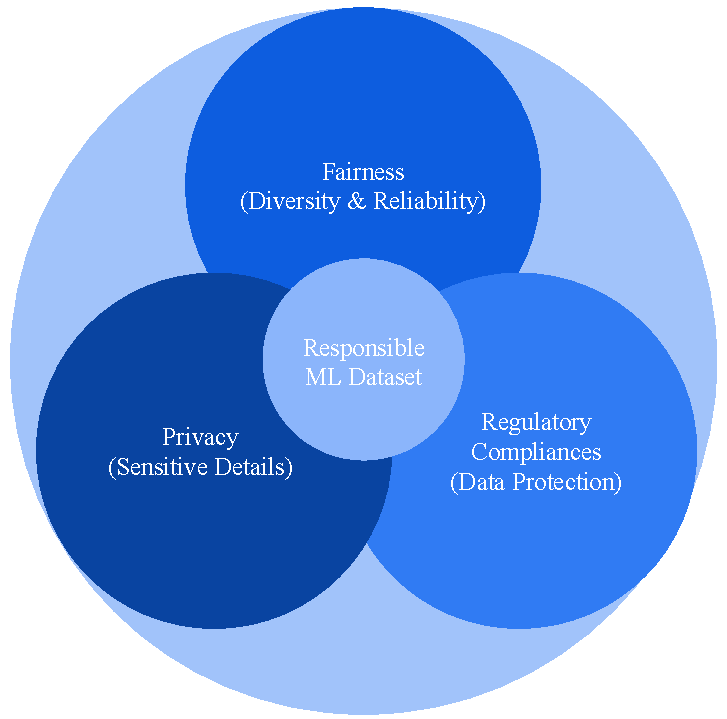
\includegraphics[width=0.5\linewidth]{images/Revised_Figure1_RMLD.pdf}
\caption{We introduce the concept of Responsible Machine Learning Datasets and propose a quantitative rubric along with recommendations for future datasets.}
\label{fig:vizabstract}
\end{figure}
% This study focuses on evaluating datasets across the three axes of fairness, privacy, and regulatory compliance.


Among the different stages of an AI system development pipeline, data collection and annotation is one of the most important ingredients which can have a significant impact on the system. Current AI algorithms are deemed \textit{data-hungry} and tend to be extremely data-driven, and any irregularities in the datasets utilized during the development of these algorithms can directly impact the learning process. Several researchers have demonstrated that non-responsible use of datasets can lead to challenges such as fairness of the model and leakage of private information such as identity information or other sensitive attributes. Certain gender and race subgroups are shown to be under-represented in face-based image datasets~\cite{cao2018vggface2,yi2014learning} while some datasets contain objects specific to certain geographies or specific contexts~\cite{deng2009imagenet,rojasdollar}. Many algorithms have also been shown to suffer from spurious correlations in the dataset~\cite{geirhos2020shortcut,li2022whac,mehta2022you}. Similarly, concerns regarding the leakage of private information from popular datasets such as ImageNet have surfaced over recent years. In order to build responsible AI systems, it is therefore important to use datasets that are responsibly curated. We assert that \textit{Responsible Datasets leads to building Responsible AI Systems}. 


 %While existing work focuses on the post-hoc evaluation of algorithms for their trustworthiness, we provide a framework that considers the data component separately for understanding its role in the algorithmic pipeline. 


% Further, AutoML tools provide power to develop these algorithms through increased resources at a reduced effort. 

% \noindent While considerable focus lies on building responsible AI through better algorithms, there is limited focus on the data used for development. For responsible AI, we require responsible datasets. 
% Such issues have been readily mitigated to a certain degree by fixing the underlying datasets to be more representative in their samples.
%Algorithms have been shown to favor males over females in job applications \cite{} while in the context of facial analytics, criminal recidivism systems have been shown to be biased against African Americans \cite{}. The Twitter algorithm favors young, white faces in its posts \cite{}. 



% \begin{figure*}[t]
% \centering
% \includegraphics[width=0.9\textwidth]{images/vizabs4.pdf}
% \caption{This study focuses on evaluating datasets across the three axes of fairness, privacy, and regulatory compliance.}
% \label{fig:vizabstract}
% \end{figure*}

Current research for understanding and evaluating trustworthiness focuses primarily on the performance of the models. However, by identifying these issues at the dataset level, we can lay the ground for creating better and \textit{responsible} datasets, and better AI. With the motivation to evaluate the reliability or trustworthiness of data, in this research, we present a framework to evaluate datasets via the proposed \textit{responsible rubric} across the axes of fairness, privacy, and regulatory compliance (refer to Figure \ref{fig:vizabstract}).
%which considers the diversity, inclusivity, and reliability of annotations for fairness evaluation, vulnerable annotations that can lead to the leakage of private information for privacy evaluation, and compliance with respect to subject consent, ethics/IRB approval and facility to expunge an enrolled data point.
To the best of our knowledge, this is the first framework that quantitatively evaluates the trustability of the data used for training ML models. For defining dataset fairness, we consider the impact of three factors: diversity, inclusivity, and reliability of annotations. \textit{Inclusivity} considers whether different groups of people are present in the dataset across parameters of sex, skin tone, ethnic group, and age, and \textit{diversity} quantifies the distribution of these groups in the dataset.  


For evaluating privacy preservation in datasets, we identify vulnerable annotations that can lead to the leakage of private information. Finally, we assess datasets for their degree of compliance with contemporary regulatory norms. Different governments around the world have approved various data privacy laws in the past few years. The popular General Data Protection Regulation (GDPR)~\cite{regulation2016regulation} requires the right to erasure based on its Article 17 (denoted as [Art. 17, GDPR]) and may require the consent of data subjects [Art. 12, GDPR] among other laws for data protection. Subjects providing data should have complete knowledge as to how their data will be used, and they should have the ability to revoke their consent. Further, if a dataset contains information such as images or potentially unethical data, there should be a mechanism to report such incidents. %The recently released Ego4D datasets provide the user with the ability to flag concerns via an interactive user interface~\cite{grauman2022ego4d}.  
%With laws like GDPR gaining wide acceptance, the creation of newer datasets must be done in compliance with these laws. 
Through the axes of fairness, privacy and regulations, we demonstrate the applicability of the proposed framework by analyzing datasets from biometrics and healthcare domains, particularly face recognition and chest XRay datasets. After surveying over 100 datasets and discarding datasets unusable for this study
because of their small size or unavailability, we utilized a total of 60 datasets. Some of our key observations are as follows: 
\begin{itemize}
    \item Most of the existing datasets suffer on all three axes of \textit{fairness}, \textit{privacy} and \textit{regulatory compliance}, as per the proposed rubric. 
    \item Fairness is a major concern for most of the datasets we surveyed.
    \item Most existing datasets do not focus on regulatory compliances.
    \item Our analysis highlights that curating datasets from the web poses major risks to privacy preservation.
    \item  We also observe the \textit{fairness-privacy paradox} that exists in the development of datasets where the presence of sensitive attributes aids fairness evaluation but potentially leaks a subject’s private information.
\end{itemize}

Finally, we provide recommendations for constructing datasets. These recommendations can serve as an ethical sounding board for development of responsible datasets in the future.
% The fairness in datasets is limited towards

%\todo{This can go in conclusion section}\noindent 

% Two detailed case studies are performed  in this study- face-based image datasets and chest X-ray-based medical imaging datasets. We further provide recommendations for the design of `responsible datasets.'

%%%%%%%%%%%%%%%%%%%%%%%%%%%%%%%%%%%%%%%%%%%%%%%%%%%%%%%%%%%%%%%%%%%%%%%%%%%
% % Regulatory Compliances
%%%%%%%%%%%%%%%%%%%%%%%%%%%%%%%%%%%%%%%%%%%%%%%%%%%%%%%%%%%%
\begin{table*}[]
\centering
% enforced from 2016 in the European Union
\caption{\label{tab:regulations} Some of the laws surrounding data privacy around the world other than the GDPR~\cite{regulation2016regulation}.}
\begin{tabular}{|C{0.1\textwidth}|p{0.3\textwidth}|C{0.04\textwidth}|C{0.055\textwidth}|p{0.26\textwidth}|C{0.09\textwidth}|}
\hline
\textbf{Country(s)}       & \textbf{Title of Law}                                                                       & \textbf{From} & \textbf{Amended} & \textbf{Relevant Authority}                   & \textbf{Region}                    \\ \hline
Brazil                    & General Data Privacy Law (LGPD) \cite{brazil}                                              & 2018          & 2019             & Autoridade Nacional de Proteção de Dados (ANPD)      & Latin America                      \\
India                     & Information Technology Act 2000 \cite{indiait}                                             & 2000          & 2008             & Ministry of Law and Justice                          & Asia                               \\
                          & India's Personal Data Protection Bill (PDPB) 2019 \cite{indiapdpb}                         & 2019          & 2019             & Data Protection Authority of India                   &                                    \\
Israel                    & Protection of Privacy Law of 1981 \cite{israel}                                            & 1981          & 2020             & Privacy Protection Authority (PPA)                   & Middle East                        \\
Japan                     & Act on Protection of Personal Information \cite{japan}                                     & 2003          & 2020             & Personal Information Protection Commission           & Asia                               \\
Lithuania                 & Law on Legal Protection of Personal Data \cite{lithuania}                                  & 1996          & 2018             & State Data Inspectorate                              & Europe                             \\
New Zealand               & New Zealand's 1993 Privacy Act \cite{newzealand}                                           & 1993          & 2020             & Privacy Commissioner                                 & Australiasia                       \\
Nigeria                   & Nigeria Data Protection Regulation 2019 (NDPR) \cite{nigeria}                              & 2019          & 2019             & Nigerian Information Technology Development Agency   & Africa                             \\
South Africa              & Protection of Personal Information Act (POPIA) \cite{southafrica}                          & 2013          & 2013             & Information Regulator                                & Africa                             \\
Switzerland               & Data Protection Act \cite{switzerland}                                                     & 1992          & 2020             & Federal Data Protection and Information Commissioner & Europe                             \\
Thailand                  & Personal Data Protection Act (PDPA) 2019 \cite{thailand}                                   & 1997          & 2019             & Personal Data Protection Committee                   & Asia                               \\
Turkey                    & Law 6698 on Personal Data Protection (LPDP) \cite{turkey}                                  & 2016          & 2016             & Data Protection Authority                            & Europe                             \\
USA: California & California Privacy Rights Act of 2020, amending California Consumer Privacy Act \cite{usc} & 2020          & 2020             & California Privacy Protection Agency (CPPA)          & North America                      \\
USA: Illinois   & Biometric Information Privacy Act (BIPA) \cite{bipa}                                       & 2008          & -                & U.S. Court of Appeals for the Ninth Circuit    & \multicolumn{1}{l|}{North America} \\
USA: Texas      & Texas Consumer Privacy Act (TXCPA) \cite{texas}                                            & 2019          & -                & Texas House of Representatives                       & \multicolumn{1}{l|}{North America} \\
                          & Texas Capture or Use of Biometric Identifier Act (CUBI) \cite{texascubi}                   & 2009          & 2017             & Texas Attorney General                             & \multicolumn{1}{l|}{}              \\
USA: Washington & Washington Biometric Privacy Protection Act (House Bill 1493)  \cite{washington}           & 2017          & -                & Washington State Attorney General             & \multicolumn{1}{l|}{North America} \\ \hline
\end{tabular}
\end{table*}

%%%%%%%%%%%%%%%%%%%%%%%%%%%%%%%%%%%%%%%%%%%%%%%%%%%%%%%%%%%%%%%%%%%%%%%%%%

\section{Related Work}
 % General discussion about datasets
In recent years, there has been an increasing focus on datasets being used in ML and deep learning. Specifically, such concerns are heightened when datasets pertain to the collection of sensitive data such as biometrics and medical data. According to a recent study, the importance of dataset quality being used in AI/ML is constantly undermined, and the data collection work is often undervalued in the community~\cite{sambasivan2021everyone}.

Researchers have addressed the need for data-centric AI as well as the impact of regulations and policies on trustworthy AI~\cite{liang2022advances}. Heger et al.~\cite{heger2022understanding} conducted interviews with ML practitioners and discovered the need to emphasize the relationship between data documentation and responsible AI. Scheuerman et al. identified the patterns followed in the collection process of computer vision datasets based on 1000$+$ publications and also emphasized the importance of proper dataset documentation~\cite{scheuerman2021datasets}.

There has been discussion around the collection of socio-cultural data where researchers have highlighted the need to design institutional frameworks and procedures inspired by archival data~\cite{jo2020lessons}. Some of the essential considerations are consent, inclusivity, power, transparency, ethics, and privacy. Similarly, focusing on the entire dataset development pipeline, Peng et al.~\cite{peng2021mitigating} studied nearly 1000 papers citing problematic datasets such as Labeled Faces in the Wild (LFW), MS-Celeb-1M~\textit{(decommissioned)}, and DukeMTMC~\textit{(decommissioned)}. The authors provide recommendations for dataset creators as well as conference program committees to encourage more ethical creation of datasets. 

In 2021, Gebru et al.~\cite{gebru2021datasheets} proposed a comprehensive `datasheet' detailing information about the dataset accompanying its release. The datasheets are designed to raise transparency and accountability in the datasets. On similar lines, Hutchinson et al. introduced a framework that helps build accountability and transparency in the data development process~\cite{hutchinson2021towards}. By segregating data development process into various stages, the authors described the roles played by individuals such as requirements owner, stakeholder, and reviewer at each stage. Palluda et al.~\cite{paullada2021data} promoted the usage of quantitative as well as qualitative measures for the effective development of datasets. They showcase how representational harms and spurious correlations present in the datasets can lead to unfair decisions.
% Holland et al.~\cite{holland2020dataset} perform different statistical analyses based on their data to understand any correlations between the data variables.

\noindent \textbf{Fairness in Datasets:} In order to build fairer AI, researchers have studied bias in various settings~\cite{tommasi2017deeper, yangfei2020towards, de2019does, singh2022anatomizing}. A recent report by NIST for identifying and managing bias in AI has cited the reliance on large-scale datasets as the leading cause of using unsuitable datasets for training and evaluation~\cite{schwartz2022towards}. The report discusses various challenges and factors associated with datasets in modern AI such as lack of representation, and statistical and socio-technical factors. Towards better representation in AI, Kamikubo et al. analyzed 190 accessibility datasets. Their analysis revealed harmful trends such as lack of older adults for autism, developmental and learning communities. To this end, they suggested more meaningful interactions with data contributors~\cite{kamikubo2022data}. Similarly, in the domain of NLP, some researchers have proposed the use of data statements that can help understand the intent and, specifically, the biases of the data~\cite{bender2018data}. The data statement emphasizes the inclusion of information such as the curation rationale and annotator demographic. Some researchers have proposed toolkits for evaluation of bias in the dataset which include object-based, person-based, and geography-based analyses through annotations~\cite{wang2022revise}.
% Further, some studies analyzing the geo-diversity of datasets have observed a bias towards a euro-centric representation~\cite{shankar2017no}.

\noindent \textbf{Privacy Leakage in Datasets:}
In this work, we refer to the term \textit{privacy leakage} as ``the unintended or unauthorized/accidental exposure of sensitive or protected personal data/information, which may compromise an individual's identity." The concerns of privacy leakage surrounding datasets in deep learning have grown over the past few years. In Birhane et al.~\cite{birhane2021large}, the authors discuss the issues of consent and privacy breaches in the context of large-scale vision datasets such as ImageNet. They highlight the harms associated with poor dataset curation practices and propose mandatory institutional reviews. 
% Yang et al.~\cite{yang2022study} have annotated and blurred the faces in the ImageNet dataset and show that the performance of the model, when trained on this dataset, degrades while ensuring privacy. 

In the field of security and privacy, researchers have attempted to preserve privacy by adopting different concepts, such as $k$-anonymity \cite{samarati1998protecting} and differential privacy \cite{dwork2008differential}. To quantify privacy leakage, researchers have proposed various metrics, such as $l$-diversity \cite{machanavajjhala2007diversity}, $k$-anonymity \cite{samarati1998protecting}, $t$-closeness \cite{li2006t}, and m-invariance \cite{xiao2007m}, among others. A detailed list of these metrics has been provided by Wagner et al.\cite{wagner2018technical}. These metrics are designed to capture the extent of privacy leakage from the perspective of an adversary with knowledge \cite{li2006t}, equivalent representation of sensitive attributes \cite{machanavajjhala2007diversity}, protection from homogeneity attacks \cite{samarati1998protecting}, and other reasons. 

After the introduction of $k$-anonymity \cite{sweeney2002k}, several researchers have developed techniques for facial privacy preservation. Zang et al. \cite{zhang2018privacy} devised a function to add random noise to existing data samples to synthesize new samples. This was aimed at masking sensitive information in the dataset while preserving the performance of the model. Chhabra et al. \cite{chhabra2018anonymizing} proposed an algorithm that provides the control to the user to anonymize k-facial attributes while preserving other attributes and identity information. Li et al. \cite{li2019anonymousnet} proposed a technique to anonymize identity and attribute while maintaining the data utility. The authors also performed quantification of privacy preservation through $k$-anonymity. 

In other works, researchers have used Mechanical Turk participants to identify privacy-sensitive information in images to automate the privacy attribute selection/identification task for obfuscation~\cite{li2018human}. Gervais et al.~\cite{gervais2016quantifying} propose a framework to infer the location by analysing the consumer purchase histories. Further, experiments have demonstrated the benefit of teaching algorithms to predict the presence and purpose of private information. Orekondy et al.~\cite{orekondy2017towards} propose an algorithm to predict a leakage risk score for the input image using their proposed VISPR dataset. Orekondy et al.~\cite{orekondy2018connecting} have also proposed a redaction by segmentation approach to aid users in selectively sanitizing images of private content. The proposed approach segments out the privacy attributes in images and provides privacy vs data-utility evaluation analysis. Gurari et al.~\cite{gurari2019vizwiz} propose a dataset and study visual privacy issues faced by people who are blind and are trying to learn about their physical surroundings. \\
% 
% Orekondy et al.~\cite{orekondy2017towards} proposed a dataset called the VISPR dataset that contains 68 attributes corresponding to personal information (beyond faces).
% The paper reports a taxonomy for photo privacy that describes what content is considered sensitive and how sharing preferences differ across potential photo recipients. 
% To address privacy leakage in datasets, different researchers have also proposed algorithms to preserve privacy in datasets. 

\noindent \textbf{Regulatory Compliance in Datasets:} With the increasingly high emphasis on data protection, various countries around the world have put legislation in place for data security and privacy. According to a report, 157 countries in the world had instated data privacy laws by mid-March 2022~\cite{unctad, greenleaf2021global, greenleaf2022now}. Most of these laws are influenced by GDPR~\cite{regulation2016regulation} but contain certain variations.
The GDPR may prohibit the processing of biometric data unless explicit consent from the subjects is not provided. By providing the \textit{right to be forgotten}, the GDPR puts the subject in charge of their data. Different studies have been conducted to understand the impact of GDPR on artificial intelligence~\cite{forti2021deployment, goldsteen2021data}. 
% which allows a data subject to withdraw consent at any time

In Table~\ref{tab:regulations}, we summarize data privacy laws for some of the countries around the world. There are other laws specific to certain kinds of data, such as the Health Insurance Portability and Accountability Act (HIPAA)~\cite{act1996health} for medical health in the US and the Biometric Information Privacy Act (BIPA)~\cite{bipa} protecting biometric information in the state of Illinois, US. Other US states are actively working towards enforcing their data privacy laws~\cite{newUSlaws}. The privacy implications of some of these acts have also received significant attention in the research community~\cite{nosowsky2006health}. Notably, the European Commission released \textit{Ethics Guidelines for Trustworthy AI}, which discusses the framework, foundations, and possible assessments for trustworthy AI~\cite{ethicsai}, as well as is in the process of amending and debating the Artificial Intelligence Act~\cite{euaiact} to address risks associated with AI applications. Recent work discusses the impact of the Artificial Intelligence Act on facial processing applications~\cite{hupont2022landscape}.

While different works identify different problematic aspects of dataset collection, very few works have looked at the factors of fairness, privacy, and regulatory compliance in datasets holistically. In this work, we provide quantitative as well as qualitative insight across the three factors and how data collection in AI needs to turn towards better and more responsible datasets.

%%%%%%%%%%%%%%%%%%%%%%%%%%%%%%%%%%%%%%%%%%%%%%%%%%%%%%%%%%%%%%%%%%%%%%%%


%%%%%%%%%%%%%%%%%%%%%%%%%%%%%%%%%%%%%%%%%%%%%%%%%%%%%%%%%%%%%%%%%%%%%%%%%%%%%%%%%%

\begin{table}[]
\centering
\caption{The different demographic subgroups considered for fairness quantification.}
\begin{tabular}{|p{0.08\textwidth}|p{0.35\textwidth}|}
\hline
\textbf{Demography} & \textbf{Subgroups}                                                                                                      \\ \hline
Sex                 & Male, Female, Other                                                                                                     \\ 
\multirow{3}{*}{Ethnicity}           & White/Caucasian, Black/African, Southeast Asian, East Asian, Indian, Hispanic/Latino, Middle Eastern, Mixed-race, Other \\ 
Skin tone           & Type I-VI using Fitzpatrick scale                                                                                       \\ 
\multirow{2}{*}{Age} & 0-3, 4-7, 8-15, 16-20, 21-30, 31-40, 41-50, 51-60, 61-70, 71-100                                                        \\ \hline
\end{tabular}
\label{tab:fairnessgroups}
\end{table}

% \section{Study Design}
% Should we add a section here about how many databases we picked and filtered through, why we are using face datasets etc.? Which datasets are we using and why? Can we add information here on the egocentric and medical dataset domains, maybe? How the idea of fairness, privacy, and regulatory compliance can be extended to domains such as object recognition, etc. 
% Talk about how many databases we picked. Why faces? The immense number of datasets. What do other works do?


\section{Methods}
In this section, we describe the methodology adopted for designing the framework for \textit{Responsible Datasets}. We quantify datasets across the axes of fairness, privacy, and regulatory compliance. The concerns regarding these factors may vary from domain to domain. For example, fairness in a face image dataset may differ from those in an object or egocentric dataset. The quantification in this section is based on datasets centered around individuals and specifically, face-based datasets.
% However, we believe that the basic notion of quantification described in this section is extensible to datasets of different domains. \\

\subsection{Quantifying Dataset Fairness} In deep learning, fairness concerns have been raised for datasets in multiple domains in different contexts~\cite{cao2018vggface2,rojasdollar}. In face-based image datasets, some sex and race subgroups may be under-represented~\cite{cao2018vggface2,yi2014learning}. In object-based datasets, datasets may contain objects specific to certain geographies or in specific contexts~\cite{rojasdollar,deng2009imagenet}. Similarly, text-based and multi-modal datasets may suffer from spurious correlations in datasets leading to bias in the performance of trained models~\cite{geirhos2020shortcut}.

In this work, we consider the impact of three factors for quantification of dataset fairness- diversity, inclusivity, and labels (See Fig.~\ref{fig:fairformula}). In the context of face-based datasets, \textit{inclusivity} quantifies whether different groups of people are present in the dataset across parameters of sex, skin tone, ethnic group, and age. \textit{Diversity} quantifies the distribution of these groups in the dataset, with an assumption that a balanced dataset is the most fair. While a balanced dataset does not guarantee equal performance, existing work has shown improved fairness with the use of balanced datasets \cite{wang2021meta, ramaswamy2020fair}. We note that such a dataset may not be ideal in many cases, but it acts as a simplifying assumption for the proposed formulation. Finally, we consider the reliability of the \textit{labels} depending on whether they have been self-reported by the subjects in the dataset or are annotated based on apparent characteristics. 

We consider four demographic groups- \textit{sex}, \textit{skin tone}, \textit{ethnicity}, and \textit{age}. The different subgroups considered for these demographics are specified in Table~\ref{tab:fairnessgroups}. We utilize the information regarding the biological sex of an individual while leaving room for error in the class \textit{Other}. For ethnic subgroups, we take inspiration from the FairFace dataset~\cite{karkkainen2021fairface} with the addition of the mixed-race as a separate category. Ethnicity subgroups around the world tend to be extremely variable. We have adopted the maximum ethnic subgroups as represented in the literature by the FairFace dataset. The age subgroup classification is based on the categories in the AgeDB dataset~\cite{moschoglou2017agedb}. The age annotations were binned as per AgeDB categorization for datasets that provided continuous age values.

The proposed formulation for quantification of fairness in a dataset is dependent on the annotations available in a dataset (See Fig.~\ref{fig:fairformula}). Let \textbf{D} = \{sex, skintone, ethnicity, age\} denote the complete set of demographics considered for evaluation of any dataset, and \textbf{S} denote the corresponding subgroups in each demographic (Refer Table \ref{tab:fairnessgroups} for subgroups considered for each demographic). Then, $\textbf{D}_1$ = sex, and $\textbf{S}_1$= \{male, female, other\}. For a given dataset, \textbf{d} denotes the set of demographics annotated in the dataset, and \textbf{s} denotes the subgroups corresponding to those demographics. For example, for the AgeDB dataset \cite{moschoglou2017agedb}, \textbf{d} = \{sex, age\}, and $\textbf{s}_i$ = \{male, female\} for $ith$ demographic in \textbf{d}, and  $\textbf{s}_{ij}$ = male for $jth$ subgroup of $ith$ demographic $(i=1, j=1)$. Then, the \textbf{inclusivity} $r_i$ for each demography is defined as the ratio of demographic subgroups present in the dataset and the pre-defined demographic subgroups in $\textbf{S}_i$. This is quantified as-
\begin{equation}
     r_i = 	|s_i|/|S_i|
\end{equation}

The \textbf{diversity} $v_i$ is calculated using Shannon's diversity index~\cite{shannon1948mathematical} to capture the distribution of different subgroups for a given demography. 
\begin{gather}
    p_{ij} = num(s_{ij})/\sum_j{num(s_{ij})}  \\
    v_i = - \sum_j{p_{ij} * ln(p_{ij})},
\end{gather}

where $num(\textbf{s}_{ij})$ denotes the number of samples for the $jth$ subgroup of the $ith$ demographic in the dataset. In certain cases where the number of samples is not available, we consider $num$ to denote the number of subjects in the dataset. Fairness across each of the demographics is measured between 0 to 1. For example, if a dataset contains images corresponding to each of the six skin tones, it will have an inclusivity score of 6/6 = 1, and if the number of samples is balanced across each of the subgroups of skin tone, the diversity score will also be 1. When combined, that will provide an overall score of 1*1 = 1. By multiplying the inclusivity and diversity scores, we are providing information about the presence as well as distribution of samples corresponding to a given demographic. These scores are added for the four demographic attributes.

The \textbf{label score} $l$, is then calculated based on whether the labels or annotations for the dataset are self-reported, classifier-generated, or apparent. \textit{Self-reported labels} indicate that the subjects provided their demographic information as a part of the data collection process. \textit{Classifier-generated labels} imply that the demographic labels were obtained through an automated process of classification. Finally, \textit{apparent labels} indicate that the annotations were done by an external annotator after observing the images (for example, through Amazon Mechanical Turk). Based on the type of annotations, a \textit{label score} is assigned for the dataset between 0 to 1, with self-reported labels assigned a value of 1, classifier-generated labels assigned 0.67, and apparent labels assigned a value of 0.33. machine-generated labels, sometimes referred to as {\em pseudo labels}, are assigned a higher score since they have been shown to be more reliable than human-annotated labels for use in deep learning-based applications \cite{lee2013pseudo, tuan2017regressing, chang2019deep}. We acknowledge that there may be different perceptions of reliability in annotation based on the task and nature of the data. However, the labels generated by a trained classifier are consistent while that may not be true for human annotators. Based on this rationale, we assign a higher score to classifier-generated labels. 

In cases where the labels are collected using more than one of the three categories, an average of the corresponding categories' scores is taken. For medical datasets, a score of 1 is provided if a medical professional provides/validates the annotations, else a score of 0 is provided. The label score is provided for the entire dataset as per the current formulation. To calculate the \textbf{fairness score}, $F$, for the dataset, the factors of inclusivity, diversity, and labels are combined as follows,
\begin{equation} \label{eq:fairnessquant}
    F = \sum_i{(r_i * (1 - v_i))} + l
\end{equation}
The fairness score is designed such that a higher value indicates a fairer dataset while a lower value indicates a less fair dataset.

\begin{figure*}[]
\centering
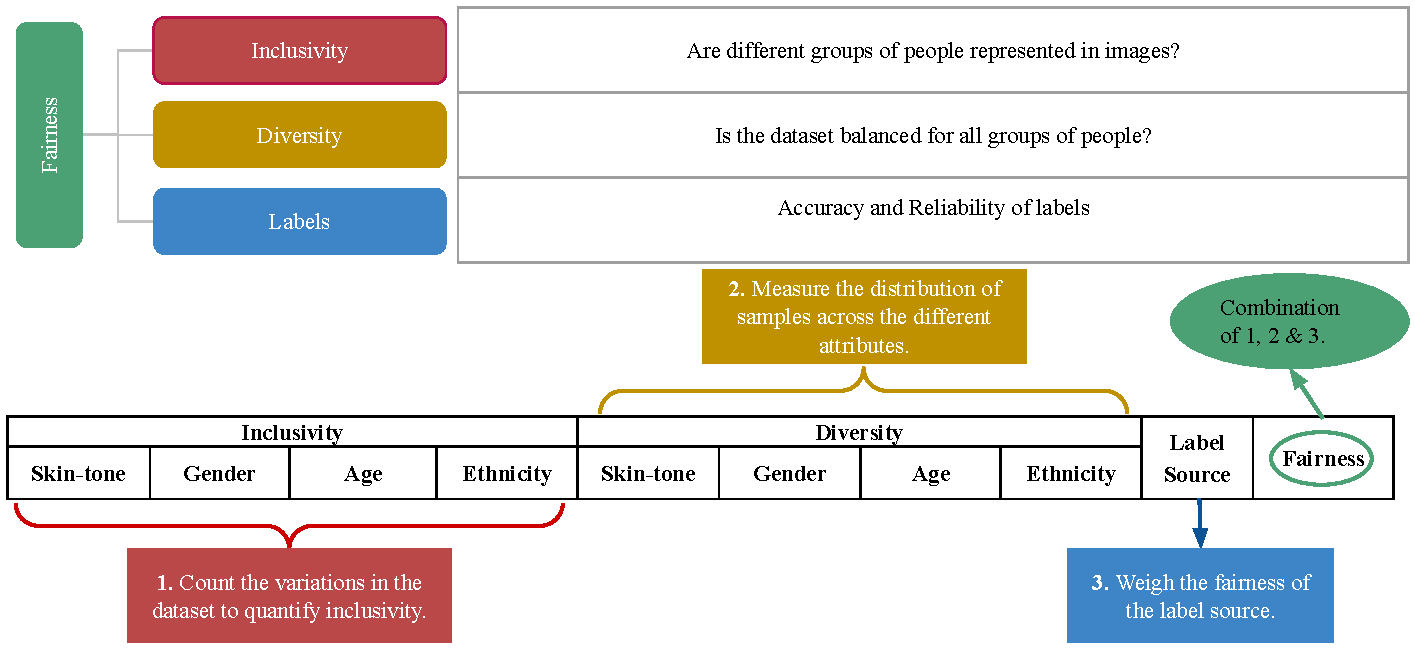
\includegraphics[width = 0.97\textwidth]{images/FairnessQuantificationUpdated.pdf}
\caption{(Top) The three aspects involved in fairness quantification- Inclusivity, Diversity, and Labels, and the questions they answer. (Bottom) The formulation employed for the calculation of the fairness score.}
\label{fig:fairformula}
\end{figure*}

% % old
% Let the number of samples in the dataset be $n$. In certain cases where the number of samples are not available, we consider $n$ to denote the number of subjects in the dataset. Let $d_{sex}$, $d_{skintone}$, $d_{ethnicity}$, and $d_{age}$ represent the different demographics for which we evaluate a certain dataset. Then for each demography $d_i$, there are subgroups present in $d_i$, denoted by $s_i$. For example, for $d_{sex}$, the corresponding $s_{sex} = \{male, female, other\}$. Then, the samples in the dataset corresponding to the \textit{male sex} may be represented as $s_{sex\_male}$. Let $S_i$ denote the complete set of subgroups corresponding to each $d_i$ $\forall i$. 
% where $j$ is used to represent the different subgroups in a demography $d_i$.

\subsection{Quantifying Dataset Privacy} Deductions and attacks can be carried out using the annotated labels in publicly available supervised datasets (See Figure \ref{fig:privacy}). Annotated attributes in a face dataset, for example, can be used for face profiling~\cite{findface, facepp, socialmapper, gnanasekar2019face}. In contrast, vehicle registration numbers from location datasets can be used to make malicious deductions and track someone down~\cite{orekondy2017towards,5958033}. As a result, the more annotations there are in the dataset, the more privacy is potentially leaked. The extent of privacy leakage can be summarised in terms of the quantity of information leaked and the extent to which private information is exposed in the annotated labels. 

\noindent In this work, for quantification of privacy leakage in the publicly available datasets, we identify vulnerable label annotations that can lead to the potential leakage of private information and devise a mathematical formulation. This formulation employs the dataset's annotated labels to quantify the potential privacy leakage. We identify six label annotations that are widely available in the datasets and lead to leakage of privacy in datasets: \textit{name identification}, \textit{sensitive and protected attributes}, \textit{accessories}, \textit{critical objects}, \textit{location inference}, and \textit{medical condition}. 
Let the set $A$ constitute these identified attributes, i.e.:

\begin{equation}
    A = \{A_N, A_{SP}, A_{AC}, A_C, A_L, A_M\}
\end{equation}
% add for user consent here.

The attributes used in defining $A$ are as follows:
% Each of the attributes listed above is described below:
\begin{itemize}
    \item \textit{Name Identification Information $A_N$:} This attribute refers to the name of each individual annotated in the dataset. This annotation potentially leads to the highest level of privacy leakage.
    \item \textit{Sensitive and Protected Attribute Information $A_{SP}$:} These attributes refer to information regarding gender, sexual orientation, race, past records, etc., corresponding to an individual.
    \item \textit{Accessory Information $A_{AC}$:} This attribute denotes the presence of accessories such as hats and sunglasses in a face image as well as other attributes such as five 'o'clock shadow. 
    \item \textit{Critical Objects $A_C$:} This attribute denotes the presence of objects revealing the identity of a person, such as credit cards or signatures.
    \item \textit{Location Information $A_L$:} This attribute denotes the presence of information in the image that can potentially disclose a person's location, such as geographical coordinates or popular landmarks in the image background.
    \item \textit{Medical Condition Information $A_M$:} This attribute denotes the presence of any information regarding the medical condition of an individual in the dataset.
\end{itemize}

For a dataset, we manually check for the presence of the annotations from the aforementioned list to estimate its privacy leakage, and a point is awarded for each attribute annotation. The privacy leakage score ($PL$) is then calculated as the sum of all the present attributes as described below:

\begin{equation}
    PL =\sum_{i=1}^{6} A_i.
\end{equation}

Finally, the \textbf{privacy preservation score}, $P$, for a given dataset is estimated as,
\begin{equation}
    P = (|A| - PL).
\end{equation}

$P$ indicates the amount of information being preserved in a dataset and represents its dependability for public use. We note that while the presence of these annotations constitutes privacy leakage in our formulation, it aids the computation of the fairness score described in the previous section. We discuss this fairness-privacy paradox in detail later in the text.

% Malicious deductions may be made through one or more of the aforementioned annotations, resulting in the privacy leakage of private data present in the dataset. For instance,  using the annotations from a medical dataset, it is possible to identify any person included in the dataset based on residence. 

%%\textbf{Write the formulation here and describe it.}

% Some of them are listed in Table \ref{tab:lawsworld}.
\subsection{Quantifying Regulatory Compliance} Different countries around the world have approved various data privacy laws in the past few years. One of the most widely accepted documents covering data privacy laws is the one applicable in European countries known as the GDPR~\cite{regulation2016regulation}. The following laws can be applied to deep learning methodologies and/or datasets,
\begin{itemize}
    \item Right to be forgotten (right to erasure) [Art. 17]
    \item Consent of data subjects [Art. 12]
    \item Right to object/restriction to the processing of their data [Art. 5, 6, 9, 18, 19]
    \item Right to rectification [Art. 16]
    \item Right of access by the data subject [Art. 15]
    \item Right to object and automated individual decision-making [Art. 21 and 22] [Recital 71]
    \item Right to lodge complaint [Art. 77]
    \item Right to effective judicial remedy [Art. 78,79]
\end{itemize}
\noindent Some of these laws restrict the use of users' personal data unless their consent is available for that particular application [Art. 5, 6, 9, 18, 19]. Other laws and conditions specified in the GDPR include,
\begin{itemize}
    \item Right to data portability [Art. 20]
    \item Security of personal data [Art. 32, 33, 34]
    \item Conditions for consent [Art. 7]
    \item Conditions for protection of children's personal data [Art. 8]
    \item Requirements for regular data protection impact assessments (DPIA) [Art. 35]
    \item Cryptographic protection of sensitive data  
    \item Breach notification requirements. [Art. 33]
\end{itemize}
% Discuss some of the laws along with the use cases.

%%%%%%%%%%%%%%%%%%%%%%%%%%%%%%%%%%%%%%%%%%%%%%%%%%%%%%%%%%%%
\begin{figure}[t]
\centering
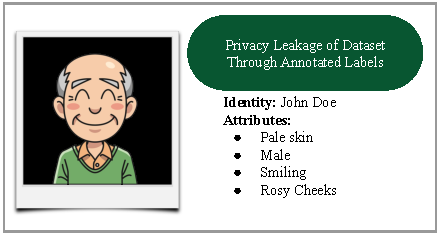
\includegraphics[width=0.43\textwidth]{images/PrivacyQuantification.pdf}
\caption{Privacy leakage through the information available in datasets. The sample is representative of information present in datasets such as the LFW dataset \cite{huang2008labeled, liu2015deep}.}
\label{fig:privacy}
\end{figure}
%%%%%%%%%%%%%%%%%%%%%%%%%%%%%%%%%%%%%%%%%%%%%%%%%%%%%%%%%%%%

Apart from the laws specified above, datasets in deep learning can benefit from existing mechanisms for institutional approval (such as IRB) and newer requirements set by popular conferences such as ethics and impact statement for datasets~\cite{EthicsCVPR}. In this paper, the \textbf{regulatory compliance score}, $R$,  in the dataset is quantified based on three factors- institutional approval (yes/no: the numerical value of 1/0), the subject's consent to the data collection (yes/no: the numerical value of 1/0), and the facility for expungement/correction of the subject's data from the dataset (yes/no: the numerical value of 1/0). If a dataset satisfies all three criteria, a compliance score of $3$ is provided. While the absence of a data subject's consent may not necessarily breach regulatory norms, for lack of a more subtle evaluation, we utilize \textit{subject consent} in the dataset as one of the factors for compliance. For example, the privacy rule in HIPAA compliance does not restrict the distribution of de-identified health data. The different factors for compliance are manually validated via information present in the published paper, webpage, and/or GitHub page for the dataset. Unless the information is explicitly specified in the aforementioned resources, it is assumed to be absent in which case we assign a value of zero. 

\begin{figure*}[!]
\centering
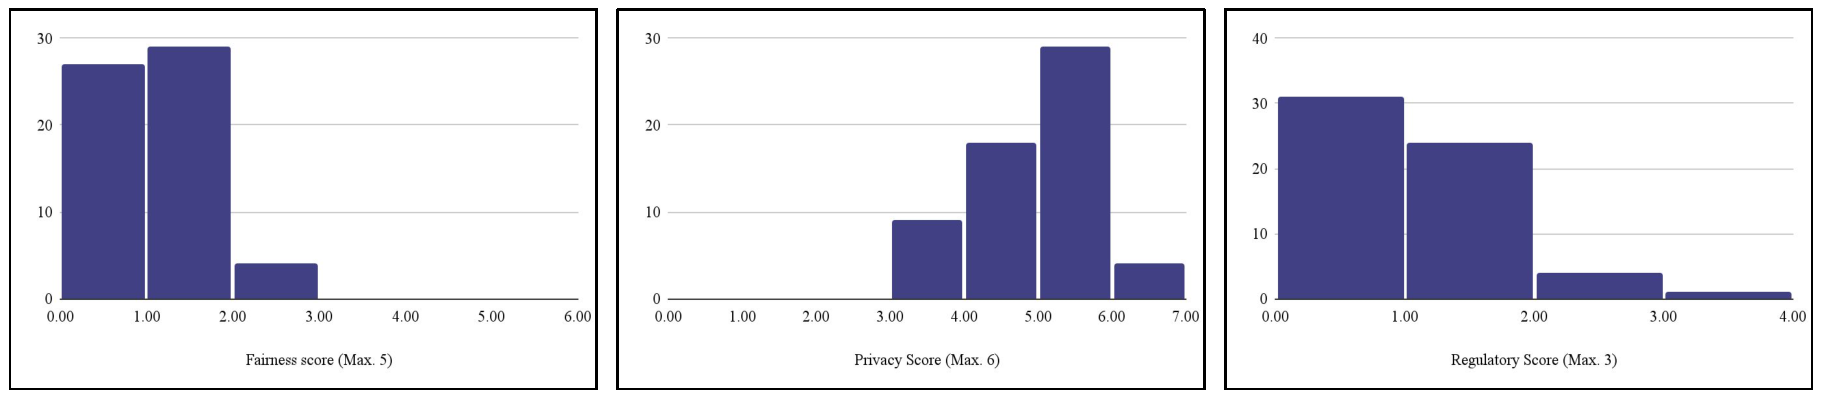
\includegraphics[width=\textwidth]{images/barplot_summary2.pdf}
\caption{The summary of fairness, privacy, and regulatory compliance scores through histogram visualization for the datasets we surveyed. (Left) The maximum value of the fairness score that can be obtained is 5, but it is observed that the fairness scores do not exceed a value of 3. (Middle) While most datasets in our study preserve privacy in terms of not leaking location or medical information, very few provide perfect privacy preservation. (Right) Most datasets comply with no regulatory norm or only one. We can observe from this plot that most datasets provide a low fairness score and perform poorly on the regulatory compliance metric.}
\label{fig:barplotsummary}
\end{figure*}

% \begin{figure}[t]
% \centering
% \includegraphics[width = 0.97\textwidth]{images/FairnessFactors.pdf}
% \caption{Classification of fairness of datasets into categories of inclusivity, diversity, and labels.}
% \label{fig:fairclassification}
% \end{figure}

%%%%%%%%%%%%%%%%%%%%%%%%%%%%%%%%%%%%%%%%%%%%%%%%%%%%%%%%%%%%

\begin{figure*}[!t]
\centering
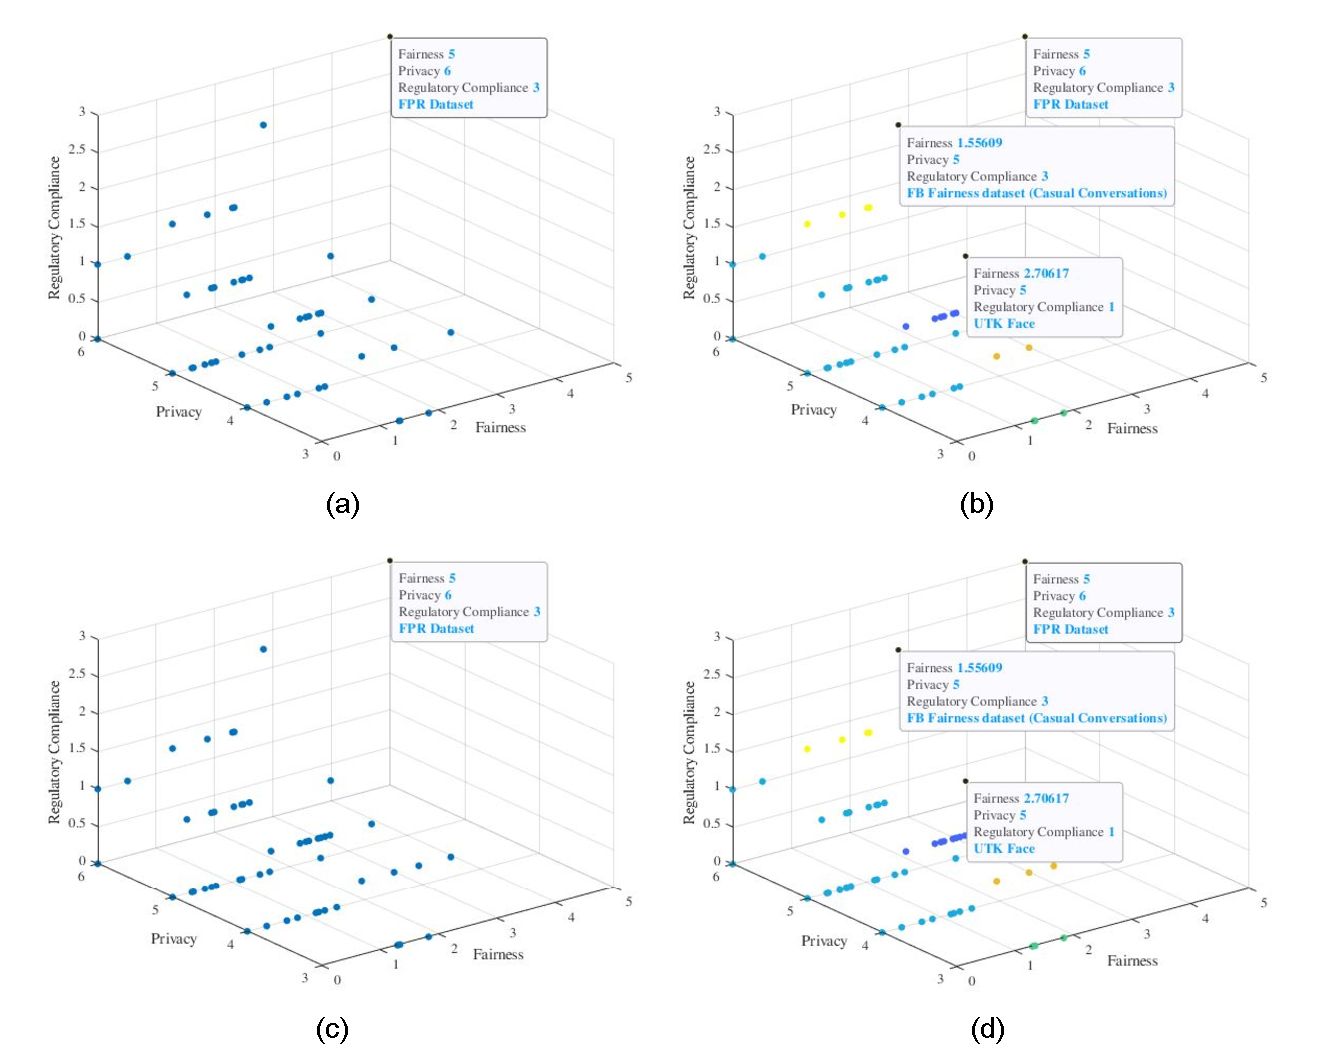
\includegraphics[width=0.8\textwidth]{images/new_cluster_analysis_wwo_medical.pdf}
\caption{Cluster analysis based on the 3-tuple quantification of fairness, privacy, and regulatory compliance for (a-b) only face-based datasets and (c-d) jointly with medical datasets. (a, c) The 3-D scatter plot of the different datasets across the three axes with the \textit{FPR dataset} plotted with perfect fairness, privacy preservation, and regulatory compliance. (b, d) The scatter plot after performing DBSCAN clustering with $eps=1$. We observe that the FB Fairness Dataset and the UTKFace dataset lie the closest to the \textit{FPR dataset}. }
\label{fig:clusteranalysis}
\end{figure*}
% (c) The same plot with a different viewing angle for clarity in cluster formation. The plot showcases six datasets in the same cluster as the `ideal dataset,' namely FB Fairness, UTKFace, LAOFIW, 10k US Adult Faces Database, CAFE and the IISCIFD datasets.

\begin{table*}[!t]
\caption{\label{tab:fprsummary}Summary of the different scores obtained for fairness, privacy, and regulatory compliance quantification obtained for the biometric datasets in the study. As can be clearly seen, the highest weighted average for fairness, privacy, and regulatory compliance is obtained on the FB Fairness dataset (Casual Conversations).}
\centering
\begin{tabular}{|p{0.4\textwidth}|C{0.11\textwidth}|C{0.11\textwidth}|C{0.11\textwidth}|C{0.11\textwidth}|}
\hline
\textbf{Dataset Name}                                                                    & \textbf{Fairness score (Max. 5)} & \textbf{Privacy Score (Max. 6)} & \textbf{Regulatory Score (Max. 3)} & \textbf{Weighted Average} \\ \hline
MORPH \cite{ricanek2006morph}                                                           & 2.2045                           & 3                               & 1                                  & 0.4247                    \\
Caltech 10K Web Faces \cite{caltech10kfaces}                                            & 0.0000                           & 6                               & 0                                  & 0.3333                    \\
FaceTracer \cite{kumar2008facetracer}                                                   & 0.6791                           & 4                               & 0                                  & 0.2675                    \\
CMU Multi-PIE \cite{ryan2009automated}                                                  & 0.2463                           & 5                               & 1                                  & 0.4053                    \\
PubFig \cite{kumar2009attribute}                                                        & 1.3349                           & 3                               & 0                                  & 0.2557                    \\
Plastic surgery database \cite{singh2010plastic}                                        & 0.0000                           & 5                               & 0                                  & 0.2778                    \\
Texas 3D Face recognition database \cite{gupta2010texas}                                & 1.1835                           & 5                               & 1                                  & 0.4678                    \\
ChokePoint \cite{wong2011patch}                                                         & 0.5097                           & 6                               & 1                                  & 0.4784                    \\
SCFace \cite{grgic2011scface}                                                           & 1.8257                           & 3                               & 0                                  & 0.2884                    \\
YouTube Faces \cite{wolf2011face}                                                       & 0.0000                           & 5                               & 0                                  & 0.2778                    \\
EGA \cite{riccio2012ega}                                                                & 0.7141                           & 5                               & 1                                  & 0.4365                    \\
10k US Adult Faces Database \cite{bainbridge2013intrinsic}                              & 0.5966                           & 5                               & 2                                  & 0.5398                    \\
Denver Intensity of Spontaneous Facial Action (DISFA) Database \cite{mavadati2013disfa} & 1.2085                           & 5                               & 1                                  & 0.4695                    \\
IMFDB-CVIT \cite{setty2013indian}                                                       & 1.3205                           & 3                               & 0                                  & 0.2547                    \\
SiblingsDB Database HQ Faces \cite{vieira2014detecting}                                 & 1.2643                           & 4                               & 1                                  & 0.4176                    \\
SiblingsDB Database LQ Faces \cite{vieira2014detecting}                                 & 0.6706                           & 5                               & 0                                  & 0.3225                    \\
Stirling 3D Face Dataset \cite{stirlingdb}                                              & 1.0040                           & 4                               & 1                                  & 0.4003                    \\
Adience \cite{eidinger2014age}                                                          & 0.5543                           & 5                               & 0                                  & 0.3147                    \\
CACD \cite{chen2014cross}                                                               & 1.2337                           & 3                               & 1                                  & 0.3600                    \\
CelebA \cite{liu2015deep}                                                               & 1.2262                           & 4                               & 0                                  & 0.3040                    \\
FaceScrub \cite{ng2014data}                                                             & 0.6670                           & 5                               & 0                                  & 0.3222                    \\
LFWA \cite{liu2015deep}                                                                & 1.3276                           & 3                               & 0                                  & 0.2552                    \\
MOBIO - Mobile Biometry Face and Speech Database \cite{tresadern2012mobile}             & 1.0501                           & 5                               & 1                                  & 0.4589                    \\
CAFE - The Child Affective Face Set \cite{lobue2015child}                               & 1.0261                           & 5                               & 2                                  & 0.5684                    \\
UFI - Unconstrained Facial Images \cite{lenc2015unconstrained}                          & 0.0000                           & 5                               & 0                                  & 0.2778                    \\
AFAD \cite{niu2016ordinal}                                                              & 1.1887                           & 5                               & 0                                  & 0.3570                    \\
IMDB-Wiki \cite{rothe2018deep}                                                          & 0.6797                           & 3                               & 1                                  & 0.3231                    \\
AgeDB \cite{moschoglou2017agedb}                                                        & 0.8603                           & 4                               & 0                                  & 0.2796                    \\
Large Age-Gap Database (LAG) \cite{bianco2017large}                                     & 0.3333                           & 4                               & 0                                  & 0.2444                    \\
PPB \cite{buolamwini2018gender}                                                         & 1.3274                           & 4                               & 0                                  & 0.3107                    \\
The IST-EURECOM Light Field Face Database \cite{sepas2017eurecom}                       & 1.2160                           & 4                               & 1                                  & 0.4144                    \\
UTK Face \cite{zhang2017age}                                                            & 2.7062                           & 5                               & 1                                  & 0.5693                    \\
VGGFace2 \cite{cao2018vggface2}                                                         & 0.0000                           & 4                               & 0                                  & 0.2222                    \\
Disguised Faces in the Wild (DFW) \cite{kushwaha2018disguised}                          & 0.0000                           & 6                               & 0                                  & 0.3333                    \\
IJB-C \cite{maze2018iarpa}                                                              & 2.1279                           & 4                               & 1                                  & 0.4752                    \\
IMDB-Face \cite{wang2018devil}                                                          & 0.4067                           & 4                               & 1                                  & 0.3604                    \\
LAOFIW \cite{alvi2018turning}                                                           & 0.0000                           & 5                               & 2                                  & 0.5000                    \\
RFW \cite{wang2019racial}                                                               & 1.4959                           & 5                               & 0                                  & 0.3775                    \\
VIP\_attribute Dataset \cite{dantcheva2018show}                                         & 0.6667                           & 5                               & 0                                  & 0.3222                    \\
AAF \cite{cheng2019exploiting}                                                          & 0.7449                           & 5                               & 0                                  & 0.3274                    \\
BUPT-Balancedface \cite{shi2020pv}                                                      & 0.3333                           & 5                               & 0                                  & 0.3000                    \\
BUPT-GlobalFace \cite{shi2020pv}                                                        & 0.3595                           & 5                               & 0                                  & 0.3017                    \\
DroneSURF \cite{kalra2019dronesurf}                                                     & 0.0000                           & 6                               & 1                                  & 0.4444                    \\
FairFace \cite{karkkainen2021fairface}                                                  & 2.5357                           & 5                               & 0                                  & 0.4468                    \\
Indian Institute of Science Indian Face Dataset (IISCIFD) \cite{katti2019you}           & 1.0570                           & 5                               & 2                                  & 0.5705                    \\
Injured Face v2 (IF-V2) database \cite{majumdar2019subclass}                            & 0.0000                           & 5                               & 0                                  & 0.2778                    \\
SOF dataset \cite{afifi2019afif4}                                                       & 1.3183                           & 5                               & 1                                  & 0.4768                    \\
BFW \cite{robinson2020face}                                                             & 0.6667                           & 5                               & 1                                  & 0.4333                    \\
DiveFace \cite{morales2020sensitivenets}                                                & 1.6636                           & 5                               & 0                                  & 0.3887                    \\
\textbf{FB Fairness dataset (Casual Conversations)} \cite{hazirbas2021towards}                   & 1.5561                           & 5                               & 3                                  & \textbf{0.7149}                    \\
MAAD-Face \cite{terhorst2021maad}                                                       & 0.9022                           & 4                               & 1                                  & 0.3935                    \\
Sejong Face Database (SFD) \cite{cheema2021sejong}                                      & 1.0566                           & 4                               & 1                                  & 0.4038                    \\ \hline
\end{tabular}
\end{table*}

\begin{table*}[]
\caption{\label{tab:fprsummarymedical}Summary of the different scores obtained for fairness, privacy, and regulatory compliance quantification obtained for the medical datasets in the study. The chest Xray datasets in this study provide a poor regulatory compliance score. The highest weighted average for fairness, privacy and regulatory compliance is obtained on the Montgomery County chest X-ray set (MC).}
\centering
\begin{tabular}{|p{0.34\textwidth}|C{0.13\textwidth}|C{0.13\textwidth}|C{0.13\textwidth}|C{0.13\textwidth}|}
\hline
\textbf{Dataset Name}                                                   & \textbf{Fairness score (Max. 5)} & \textbf{Privacy Score (Max. 6)} & \textbf{Regulatory Score (Max. 3)} & \textbf{Weighted Average} \\ \hline
\textbf{Montgomery County chest X-ray set (MC)} \cite{jaeger2014two}            & 1.4164                           & 4.00                            & 1.00                               & \textbf{0.4278}                    \\
Shenzhen chest X-ray set \cite{jaeger2014two}                          & 1.3300                           & 4.00                            & 1.00                               & 0.4220                    \\
ChestX-ray8 (NIH) \cite{wang2017chestx}                                & 1.1740                           & 4.00                            & 0.00                               & 0.3005                    \\
RSNA Pneumonia Challenge \cite{shih2019augmenting}                     & 1.1478                           & 5.00                            & 0.00                               & 0.3543                    \\
CheXpert (Stanford University) \cite{irvin2019chexpert}                & 1.5318                           & 4.00                            & 0.00                               & 0.3243                    \\
PadChest (University of Alicante) \cite{bustos2020padchest}            & 1.2094                           & 4.00                            & 1.00                               & 0.4140                    \\
BIMCV+ dataset \cite{vaya2020bimcv}                                    & 1.6556                           & 3.00                            & 1.00                               & 0.3882                    \\
COVID-19 Image Data Collection (CIDC) \cite{cohen2020covidProspective} & 1.2922                           & 3.00                            & 0.00                               & 0.2528                    \\ \hline
\end{tabular}
\end{table*}


\section{Results}
For this work, we surveyed a large number of datasets. Datasets containing human subjects were selected for the study. While fairness and privacy issues persist across different data domains such as objects and scenes \cite{rojasdollar,deng2009imagenet}, current regulatory norms are designed for people. While it is possible to extend the concepts presented in this study to other domains, we limit our discussion to face-based and medical imaging datasets.  After filtering through a total of 100 datasets and discarding datasets that are decommissioned, small in size (less than 100 images), and whose data could not be downloaded/accessed/requested, we were left with 60 datasets. These 60 datasets are used for the analysis and quantification of the responsible rubric. We use 52 face-based biometric datasets (Table \ref{tab:datasetdetails}), and eight chest Xray based medical datasets (Table \ref{tab:medicaldatasetdetails}). For face-based datasets, we filtered through over 120 datasets removing datasets that had been decommissioned, older than 2010, and whose data was inaccessible. For chest Xray datasets, we similarly surveyed through about 20 datasets before obtaining the eight analyzed in this work. We quantify the datasets across the dimensions of fairness, privacy, and regulatory compliance. Using the specified quantification methodology, we obtain a 3-tuple containing scores across the three dimensions. Analysis across the three different dimensions has been obtained through Fig.~\ref{fig:barplotsummary} where the distribution of scores has been plotted.\\
% An overview of the factors involved in performing analysis are provided in Fig. \ref{fig:vizabstract}. 

\noindent \textbf{Fairness in Datasets:} The fairness of datasets is calculated based on Eqn. \ref{eq:fairnessquant}. Representative and balanced datasets have been shown to provide fairer performance across different demographic subgroups \cite{wang2021meta}. The fairness metric described in this work provides a maximum value of 5, with five being the fairest. The average value for the fairness score obtained for the datasets comes out to be 0.96 $\pm$ 0.64, signifying that, on average, the fairness score of a dataset ranges from 0.32 to 1.6. The detailed results are provided in Tables ~\ref{tab:fprsummary} and ~\ref{tab:fprsummarymedical} for biometric and medical datasets, respectively. The UTKFace dataset is observed to be the fairest, with a score of 2.71 among the datasets listed here, providing maximum representation. It should be noted that with a maximum score of 5, the UTKFace dataset achieves slightly more than half that score. Interestingly, the average fairness score for the eight medical datasets was 1.34 $\pm$ 0.17 while the same score for biometric datasets came out to be 0.90 $\pm$ 0.67.\\

\noindent \textbf{Privacy Preservation in Datasets:} The privacy preserved in datasets is computed based on the presence of privacy-compromising information in the annotations, such as names of subjects and the presence of critical objects such as credit cards. A $P$ indicating the privacy preservation capacity and $PL$ indicating privacy leakage of the dataset are calculated. The distribution of $P$ for privacy quantification is presented in Fig. \ref{fig:barplotsummary}. The best value of $P$ is 6. We observe that the DroneSURF dataset does not contain any private information, which makes it perfectly privacy-preserving. The medical datasets in the study de-identify their subjects but naturally leak information about medical conditions, while some further provide sensitive information such as location.
\\

% in our study do not leak information based on location or medical conditions. However, they do 
% On the other hand, the lack of annotation makes it impossible to quantify it for its fairness across different demographic subgroups.\\
% \footnote{The Library of Congress defines demographic groups as ``a subset of the general population, referring to the group's age, gender, occupation, nationality, ethnic background, sexual orientation, etc." ~\cite{libraryofcongress}.}

\noindent \textbf{Regulatory Compliance in Datasets: } With modern IT laws in place, the regulatory compliance of datasets is quantified based on institutional approval of the dataset, subject's consent to the data collection, facility for expungement/correction of the subject's data from the dataset. Based on these criteria, the compliance scores are calculated with a maximum value of three. The distribution of scores is provided in Fig. \ref{fig:barplotsummary}. On average, a regulatory score value of 0.58 is obtained. We observe that the FB Fairness Dataset (Casual Conversations) satisfies all regulatory compliances, thereby obtaining the maximum regulatory score, whereas most datasets provide a score of 0 or 1. \\

\noindent \textbf{Fairness-Privacy Paradox in Datasets:} Many face-based biometric datasets provide sensitive attribute information. This leads to a \textit{fairness-privacy paradox} where the presence of these annotations enables fairness quantification but leads to privacy leakage. One way to remedy the situation is by providing population statistics in the published dataset papers instead of sensitive attribute labels for each sample. However, current fairness algorithms are evaluated through sensitive attribute annotations in the dataset, and their absence can hinder the fairness evaluation process. In differential privacy-based solutions, it has been observed that the performance degradation is unequal across different subgroups~\cite{bagdasaryan2019differential}, highlighting the need for labels for fairness analysis. The \textit{fairness-privacy paradox} remains an open problem for datasets containing sensitive attribute information such as biometrics and medical imaging. With ongoing discussion regarding concerns for privacy and fairness, regulations can sometimes provide conflicting guidance on privacy laws and proposed AI laws, giving researchers and industry a reason to approach this paradox with caution in dataset development. Recent work in face recognition is exploring models trained using synthetically generated datasets\cite{qiu2021synface, melzi2023gandiffface, kim2023dcface}. However, the training of powerful generative models utilizes large face datasets. Some diffusion-based models have also been shown to replicate the training data during generation.

% In contrast, GDPR requires explicit consent from a subject before allowing their data to be used. \\

% When the aforementioned factors are studied in conjunction, we obtain a three-dimensional representation of the datasets. The 3-tuple provides insight into how responsible a dataset may be considered for downstream training. To observe the behavior of the 3-tuple visually, we plotted a 3-D scatter plot for the datasets along with a hypothetical `ideal dataset' (Fig. \ref{fig:clusteranalysis}(a)). After applying the k-means clustering algorithm with $k=3$, we observed cluster formation as shown in Fig. \ref{fig:clusteranalysis}(b) and (c). Six datasets were found to be in the same cluster as the `ideal dataset,' namely FB Fairness Dataset, LAOFIW, the UTKFace dataset, 10k US Adult Faces Database, CAFE Database and IISCIFD. This cluster consisted of the datasets in the top six highest weighted average values (Tables \ref{tab:fprsummary} and \ref{tab:fprsummarymedical}). The datasets in the remaining two clusters scored one or none on regulatory compliance and appeared to be roughly separated into two clusters of higher and lower privacy preservation. 

\noindent \textbf{Holistic View of Responsibility in Datasets:} When the aforementioned factors are studied in conjunction, we obtain a three-dimensional representation of the datasets. The 3-tuple provides insight into how responsible a dataset may be considered for downstream training. To observe the behavior of the 3-tuple visually, we plotted a 3-D scatter plot for the face datasets along with a hypothetical \textit{FPR dataset} (Fig. \ref{fig:clusteranalysis}(a)). The hypothetical FPR dataset has a perfect fairness, privacy, and regulatory score. After applying the DBSCAN algorithm with $eps=1$ (the maximum distance between two points to be considered as a part of one cluster), we observe five clusters with two outliers. The FB Fairness Dataset and the UTKFace dataset come out to be outliers with a Euclidean distance of 3.59 and 3.20 units from the \textit{FPR dataset}. 
When compared to the other clusters, we observe that FB Fairness Dataset and the UTKFace dataset lie the closest to the \textit{FPR dataset}.

Other cluster centers lie at a distance of 4.56, 4.79, 5.11, 5.20, and 5.33 units from the \textit{FPR dataset}, with the clusters containing 4, 7, 3, 32, and 4 points, respectively. The next closest cluster is formed by the LAOFIW, 10k US Adult Faces Database, CAFE Database, and IISCIFD datasets with average scores of 0.67, 5, and 2 for fairness, privacy, and regulatory compliance, respectively. Similar observations can be made when the scatter plot includes medical datasets along with the face datasets(Fig. \ref{fig:clusteranalysis}(c-d)). The  numerical results are tabulated in Tables \ref{tab:fprsummary} and \ref{tab:fprsummarymedical}. A weighted average of the three scores is calculated by dividing each score by its maximum value and then taking an average that provides a value in the range of 0 to 1 (Table \ref{tab:fprsummary}). By utilizing this average, we observe that the top three responsible datasets come out to be the FB Fairness dataset (Casual Conversations), the Indian Institute of Science Indian Face Dataset (IISCIFD), and the UTKFace dataset. A high regulatory compliance score plays an important role in the overall responsibility score of FB Fairness and IISCIFD datasets. In contrast, a high fairness score imparts UTKFace a high responsible rubric value. To summarize the observations made over the existing face datasets, we find that-
\begin{itemize}
    \item Most of the existing datasets suffer on all the three axes of \textit{fairness}, \textit{privacy} and \textit{regulatory compliance} as per the proposed metric. For example, the UTKFace dataset is among the fairest datasets but performs poorly on regulatory compliance. On the other hand, the LFWA dataset lacks on all three fronts- fairness, privacy preservation, and regulatory compliance.
    \item While many works claim fairness as the primary focus in their datasets, these datasets provide poor fairness scores on evaluation. One such example is the DiveFace dataset. The fairness quantification of datasets using our framework shows that being fair is a major concern with 91\% of the existing datasets obtaining a fairness score of two or less out of five.
    \item A vast number of large-scale  datasets in Computer Vision are web-curated without any institutional approval. These datasets are often released under various CC-BY licenses even when these datasets do not have subject consent. We found that these datasets also fares low on the fairness front since the annotations are not always reliable, posing major risks to overall data responsibility.
    \item Following regulatory norms effectively improves the responsibility rubric for a given dataset; however, most datasets are not compliant based on the available information with 89\% datasets having a compliance score of 0 or 1.
    \item When comparing fairness, privacy, and regulatory scores, it is clear that the privacy scores are higher in general. It is worth noting that privacy standards and constraints are already defined and have  existed for a few years now~\cite{regulation2016regulation}, and datasets are possibly collected with these regulations in mind. This further indicates a need for fairness and regulatory constraints that promote data collection with higher fairness and regulatory standards.  \\
\end{itemize}

%%%%%%%%%%%%%%%%%%%%%%%%%%%%%%%%%%%%%%%%%%%%%%%%%%%%%%%%%%

\noindent \textbf{Recommendations:} Based on the observations of our framework on a large number of datasets, we provide certain recommendations to aid better dataset collection in the future.
\begin{itemize}
    \item \textit{Institutional Approval, Ethics Statement, and Subject Consent:} Datasets involving human subjects should receive approval from the institutional review board (such as IRB in the United States). Future regulations may require consent from subjects to be obtained explicitly for the dataset and its intended use. 
    % Datasets should also provide an ethics/impact statement detailing the possible ethical concerns that can be raised through the usage of the dataset. 
    \item \textit{Facility for Expungement/Correction of Subject's Data:} Datasets should provide a facility to contact the dataset owners to remove and/or correct information concerning the subject. This is necessary to be compliant with data privacy laws such as GDPR. Some existing datasets already provide the facility for expungement in their datasets such as the FB Fairness Dataset, IJB-C and the UTKFace datasets. 
    \item \textit{Fairness and Privacy:} Datasets should be collected from a diverse population, and distribution across sensitive attributes should be provided while being privacy-preserving. The proposed fairness and privacy scores can aid in quantifying a dataset's diversity and privacy preservation.  
    \item \textit{Datasheet:} Datasets should curate and provide a datasheet containing information regarding the objectives, intended use, funding agency, the demographic distribution of subjects/images, licensing information, and limitations of the dataset. By specifying intended use, the data can be restricted for processing outside of intended use under the GDPR. An excellent resource for the construction of datasheets is provided by Gebru et al.~\cite{gebru2021datasheets}. We propose modifications in the datasheet by Gebru et al. by adding questions concerning fairness, privacy, and regulatory compliance in datasets (Refer Tables \ref{tab:datasheet} and \ref{tab:newdatasheet}).
\end{itemize}

\noindent \textbf{Limitations:} The formulation for quantification in this work considers a dataset fair based on the distribution of its labels.  However, we do not account for the diversity of the data such as the presence of duplicate images for particular subgroups. Further, we do not comment on equity vs equality in the distribution of images. We note that it may be desirable to have unequal distribution between groups (e.g., when one group is harder to process than others and requires more data for the model to reach equal performance across groups) for some applications. Further, the current formulation for fairness, privacy, and regulatory scores is provided for datasets constituting individuals. While object-based datasets may also suffer from fairness issues, current data regulations are designed in accordance with the impact on human individuals. We leave analysis on object-based datasets for future work. Finally, we would like to note that the recommendations and datasheets introduced in this work are intended to establish the highest standards which can be challenging to achieve given the capabilities of current technologies. These recommendations are meant to serve as a ``north star" and reaching them requires deliberate research effort. The fairness-privacy paradox remains an open problem in the community. Similarly, removing instances of data from already trained models requires \textit{unlearning} techniques, which while being actively explored, are far from being perfect.
% Therefore, the recommendations are designed to be an ethical sounding board for future dataset collection.

\section{Conclusion}

While the vast majority of the existing literature focuses on the design of trustworthy machine learning algorithms, in this work, we offer a fresh perspective for evaluating reliability through a discussion of responsible datasets with respect to fairness, privacy, and regulatory compliance. A detailed analysis is performed  for face-based and chest Xray image datasets. We further provide recommendations for the design of `responsible ML datasets.' With governments around the world regularizing data protection laws, the method for the creation of datasets in the scientific community requires revision, and it is our assertion that the proposed quantitative measures, qualitative datasheets, and recommendations can stimulate the creation of responsible datasets which can lead to building responsible AI systems.

%In this work, we study face-based datasets in the vision community and provide a framework for the quantification of a dataset's fairness, privacy, and regulatory compliance. Existing datasets are observed to lack heavily in their fairness, privacy preservation, and regulatory compliance, opening avenues for better data curation practices.  We further introduce two datasheets that encompass Gebru's original datasheets for datasets. With this study, we aim to further the conversation about better dataset practices by holistically considering and understanding the different factors of fairness, privacy, and regulatory compliance in datasets. With governments around the world regularizing data protection laws, the method for the creation of datasets in the scientific community requires revision, and it is our assertion that the proposed quantitative measures, qualitative datasheets, and recommendations can stimulate the creation of responsible datasets which can lead to building responsible AI systems.

% Please add the following required packages to your document preamble:
% \usepackage{multirow}
\begin{table*}[]
\caption{\label{tab:datasheet} Research questions to account for the preparation of datasets. Parts of this table are taken from Gebru et al.\cite{gebru2021datasheets}. The proposed questions are highlighted in \textbf{bold}.}
\centering
\begin{tabular}{|p{0.1\textwidth}|p{0.85\textwidth}|}
\hline
\textbf{Category}                                & \textbf{Research Questions}                                                                                                                                                                                               \\ \hline
\multirow{3}{*}{Motivation}                      & For what purpose was the dataset created?                                                                                                                                                                                 \\
                                                 & \textbf{Who created the dataset (e.g., which team, research group) and on behalf of which entity (e.g., company, institution, organization)?}                                                                             \\
                                                 & \textbf{Who funded the creation of the dataset?}                                                                                                                                                                          \\ \hline
\multirow{13}{*}{Composition}                    & What do the instances that comprise the dataset represent (e.g., documents, photos, people, countries)?                                                                                                                   \\
                                                 & \textbf{How many instances are there in total (of each type, if appropriate)?}                                                                                                                                            \\
                                                 & \textbf{What is the distribution of the instances with respect to the target or label?}                                                                                                                                   \\
                                                 & \textbf{Is the distribution of instances in the dataset long-tailed  with respect to the target or label?}                                                                                                                \\
                                                 & Does the dataset contain all possible instances or is it a sample (not necessarily random) of instances from a larger set?                                                                                                \\
                                                 & What data does each instance consist of?                                                                                                                                                                                  \\
                                                 & Is there a label or target associated with each instance?                                                                                                                                                                 \\
                                                 & \textbf{Is any information missing from individual instances?}                                                                                                                                                            \\
                                                 & Are relationships between individual instances made explicit (e.g., users’ movie ratings, social network links)?                                                                                                          \\
                                                 & Are there recommended data splits (e.g., training, development/validation, testing)?                                                                                                                                      \\
                                                 & Is the dataset self-contained, or does it link to or otherwise rely on external resources (e.g., websites, tweets, other datasets)?                                                                                       \\
                                                 & \textbf{If biometric (or sensitive) information is present in the instances of the dataset such as fingerprint or faces, are these annotated?}                                                                            \\
                                                 & \textbf{If the biometric (or sensitive) information is not annotated, is it discussed in detail in the accompanying research paper or elsewhere?}                                                                         \\ \hline
\multirow{5}{2cm}{Collection Process}              & If the dataset is a sample from a larger set, what was the sampling strategy (e.g., deterministic, probabilistic with specific sampling probabilities)?                                                                   \\
                                                 & \textbf{How was the data associated with each instance acquired?}                                                                                                                                                         \\
                                                 & Who was involved in the data collection process (e.g., students, crowdworkers, contractors) and how were they compensated (e.g., how much were crowdworkers paid)?                                                        \\
                                                 & \textbf{What is the demographic of the people involved in the collection and annotation process?}                                                                                                                         \\
                                                 & Over what timeframe was the data collected?                                                                                                                                                                               \\ \hline
\multirow{3}{2cm}{Preprocessing/ cleaning/ labeling} & \textbf{Was any preprocessing/cleaning/labeling of the data done (e.g., discretization or bucketing, tokenization, part-of-speech tagging, SIFT feature extraction, removal of instances, processing of missing values)?} \\
                                                 & \textbf{Was the “raw” data saved in addition to the preprocessed/cleaned/labeled data (e.g., to support unanticipated future uses)?}                                                                                      \\
                                                 & Is the software that was used to preprocess/clean/label the data available?                                                                                                                                               \\ \hline
\multirow{6}{*}{Distribution}                    & \textbf{Will the dataset be distributed to third parties outside of the entity (e.g., company, institution, organization) on behalf of which the dataset was created?}                                                    \\
                                                 & How will the dataset will be distributed (e.g., tarball on website, API, GitHub)?                                                                                                                                         \\
                                                 & When will the dataset be distributed?                                                                                                                                                                                     \\
                                                 & \textbf{Will the dataset be distributed under a copyright or other intellectual property (IP) license, and/or under applicable terms of use (ToU)?}                                                                       \\
                                                 & Have any third parties imposed IP-based or other restrictions on the data associated with the instances?                                                                                                                  \\
                                                 & Is there a repository that links to any or all papers or systems that use the dataset?                                                                                                                                    \\ \hline
\multirow{8}{*}{Maintenance}                     & Who will be supporting/hosting/maintaining the dataset?                                                                                                                                                                   \\
  & How can the owner/curator/manager of the dataset be contacted (e.g., email address)?                                                                                                                                      \\
  & \textbf{Who bears responsibility in case of a violation of rights?}                                                                                                                                                       \\
                                                 & Is there an erratum?                                                                                                                                                                                                      \\
                                                 & Will the dataset be updated (e.g., to correct labeling errors, add new instances, delete instances)?                                                                                                                      \\
                                                 & Will older versions of the dataset continue to be supported/hosted/maintained?                                                                                                                                            \\
                                                 & If others want to extend/augment/build on/contribute to the dataset, is there a mechanism for them to do so?                                                                                                              \\
                                                 & \textbf{Are there specific guidelines for derivative work such as allowed/disallowed derivatives, distribution and licensing requirements?}                                                                               \\ \hline
\end{tabular}
\end{table*}

%%%%%%%%%%%%%%%%%%%%%%%%%%%%%%%%%%%%%%%%%%%%%%%%%%%%%%%%%%%%%%%%%%%%%%%%%%%

\begin{table*}[]
\caption{\label{tab:newdatasheet} Research questions surrounding the fairness, privacy and regulatory compliance of datasets. Parts of this table are taken from Gebru et al.\cite{gebru2021datasheets}. The proposed questions are highlighted in \textbf{bold}.}
\centering
\begin{tabular}{|p{0.1\textwidth}|p{0.85\textwidth}|}
\hline
\multicolumn{1}{|l|}{\textbf{}} & \textbf{Research Questions}                                                                                                  \\ \hline
\multirow{11}{*}{Fairness}       & Does the dataset identify any subpopulations (e.g., by age, gender)?  \\
& \textbf{Which subpopulations are identified in the dataset and how many subgroups of each subpopulation are represented? (inclusivity score)}                                                \\
 & \textbf{What is the distribution of the subgroups for each of the subpopulations? (diversity score)}       \\
& What mechanisms or procedures were used to collect the data (e.g., hardware apparatuses or sensors, manual human curation, software programs, software APIs)? \\
& \textbf{How reliable is the source of annotation for subpoulations and were the labels self-reported, apparent or classifier-generated? (label score)} \\
& \textbf{Based on the annotation in the dataset for the sensitive attributes, what is the inclusivity score, diversity score, label score and the overall fairness score?}  \\
 & \textbf{Are there any correlations between the sensitive attributes or with other attributes? (shortcuts/spurious correlations)} \\ \hline
\multirow{5}{*}{Privacy}        & Does the dataset contain data that might be considered confidential (e.g., data that is protected by legal privilege or by doctor-patient confidentiality, data that includes the content of individuals’ non-public communications)?                                                                                                                                    \\
                                & Does the dataset contain data that, if viewed directly, might be offensive, insulting, threatening, or might otherwise cause anxiety?                                                                                                                                                                                                                                    \\
& Is it possible to identify individuals (i.e., one or more natural persons), either directly or indirectly (i.e., in combination with other data) from the dataset?\\
& \textbf{If the data has been de-identified, what mechanism has been used for de-identification?} \\
 & Does the dataset contain data that might be considered sensitive in any way (e.g., data that reveals race or ethnic origins, sexual orientations, religious beliefs, political opinions or union memberships, or locations; financial or health data; biometric or genetic data; forms of government identification, such as social security numbers; criminal history)? \\ \hline
\multirow{13}{*}{Regulatory}    & Were any ethical review processes conducted (e.g., by an institutional review board)? \\
& Did you collect the data from the individuals in question directly, or obtain it via third parties or other sources (e.g., websites)?\\
& Were the individuals in question notified about the data collection?  \\
& Did the individuals in question consent to the collection and use of their data? \\
 & If consent was obtained, were the consenting individuals provided with a mechanism to revoke their consent in the future or for certain uses?  \\
 & \textbf{Irrespective of consent, is there a mechanism to expunge the data of individuals on request?}\\
 & What tasks has the dataset been used for (if any) and what other tasks can the dataset be used for? \\
& Are there tasks for which the dataset should not be used?  \\
 & If the dataset relates to people, are there applicable limits on the retention of the data associated with the instances (e.g., were the individuals in question told that their data would be retained for a fixed period of time and then deleted)? \\
& \textbf{In case of an expungement request of data, what happens to the model trained using the previous data (if any)?} \\
& \textbf{Is there a mechanism to extract the data from the trained models?} \\
& Do any export controls or other regulatory restrictions apply to the dataset or to individual instances?\\
 & \textbf{Does the dataset follow the applicable data privacy laws in your region such as GDPR in EU (if any)?}  \\ \hline
\multirow{3}{*}{Future Impact}  & Has an analysis of the potential impact of the dataset and its use on data subjects (e.g., a data protection impact analysis) been conducted?                                                                                                                                                                                                                            \\
                                & Is there anything about the composition of the dataset or the way it was collected and preprocessed/cleaned/labeled that might impact future uses?                                                                                                                                                                                                                       \\
                                & \textbf{Could there be any ethical concerns raised for the data?}                                                                                                                                                                                                                                                                                                        \\ \hline
\end{tabular}
\end{table*}
%%%%%%%%%%%%%%%%%%%%%%%%%%%%%%%%%%%%%%%%%%%%%%%%%%%%%%%%%%%%%%%%%%%%%%%%%%%

% \begin{table*}[]
% \begin{tabular}{|l|c|c|c|c|c|c|c|c|}

% \begin{table*}[]
% \caption{\label{tab:datasetdetails}Table containing details of the datasets employed for the study. The \textit{Demographic Attributes} specify the annotations for attributes such as ethnicity, skin tone, age, and gender. In contrast, \textit{Other Attributes} provides a list of some of the other attributes present in the dataset. {*}Since some datasets contain up to 40 non-demographic attributes, not all are listed here.}
% \centering
% \begin{tabular}{|p{0.25\textwidth}|C{0.1\textwidth}|C{0.1\textwidth}|C{0.1\textwidth}|C{0.1\textwidth}|C{0.1\textwidth}|C{0.08\textwidth}|}

% {*}Since some datasets contain up to 40 non-demographic attributes, not all are listed here.

\begin{table*}[!t]
\caption{\label{tab:datasetdetails}Details of the biometric datasets employed for the study. The \textit{Demographic Attributes} specify the annotations for attributes such as ethnicity, skin tone, age, and gender.}
\centering
\scriptsize
\begin{tabular}{|p{0.29\textwidth}|C{0.025\textwidth}|C{0.09\textwidth}|p{0.19\textwidth}|p{0.2\textwidth}|C{0.06\textwidth}|}
\hline
\textbf{Dataset Name}                                                                    & \textbf{Year} & \textbf{Images}             & \textbf{Facial Tasks}                                                          & \textbf{Demographic Attributes}                     & \textbf{Web Collected} \\ \hline
MORPH \cite{ricanek2006morph}                                                           & 2006          & 400K                        & Recognition                                                                    & Ethnicity, Gender, Age                              & No                     \\
Caltech 10K Web Faces \cite{caltech10kfaces}                                            & 2007          & 10.5K                       & Detection                                                                      & -                                                   & Yes                    \\
FaceTracer \cite{kumar2008facetracer}                                                   & 2008          & 3.1M                        & Attribute Classification                                                       & Ethnicity, Gender, Age                              & Yes                    \\
CMU Multi-PIE \cite{ryan2009automated}                                                  & 2009          & 755K                        & Recognition                                                                    & Ethnicity, Gender                                   & No                     \\
PubFig \cite{kumar2009attribute}                                                        & 2009          & 58.7K                       & Verification                                                                   & Ethnicity, Gender, Age                              & Yes                    \\
Plastic surgery database \cite{singh2010plastic}                                        & 2010          & 900 image pairs             & Verification                                                                   & -                                                   & Yes                    \\
Texas 3D Face recognition database \cite{gupta2010texas}                                & 2010          & 1.1K                        & Recognition                                                                    & Ethnicity, Gender, Age                              & No                     \\
ChokePoint \cite{wong2011patch}                                                         & 2011          & 64.2 K images, 48 videos    & Person Recognition                                                             & Gender                                              & No                     \\
SCFace \cite{grgic2011scface}                                                           & 2011          & 4.1K                        & Recognition                                                                    & Ethnicity (Caucasian), Gender, Age                  & No                     \\
YouTube Faces \cite{wolf2011face}                                                       & 2011          & 3.4K videos                 & Recognition                                                                    & -                                                   & Yes                    \\
EGA \cite{riccio2012ega}                                                                & 2012          & 2.3K                        & Recognition                                                                    & Ethnicity, Gender, Age                              & No                     \\
MOBIO - Mobile Biometry Face and Speech Database \cite{tresadern2012mobile}             & 2012          & 75 videos                   & Recognition                                                                    & Gender                                              & No                     \\
10k US Adult Faces Database \cite{bainbridge2013intrinsic}                              & 2013          & 2.2K                        & Recognition                                                                    & Ethnicity, Gender                                   & Yes                    \\
Denver Intensity of Spontaneous Facial Action (DISFA) Database \cite{mavadati2013disfa} & 2013          & 130K                        & Expression Recognition                                                         & Ethnicity, Gender                                   & No                     \\
IMFDB-CVIT \cite{setty2013indian}                                                       & 2013          & 34.5K                       & Recognition                                                                    & Ethnicity (Indian), Gender, Age                     & Yes                    \\
Stirling 3D Face Dataset \cite{stirlingdb}                                              & 2013          & 2K (subset)                 & 3D Reconstruction                                                              & Gender                                              & No                     \\
Adience \cite{eidinger2014age}                                                          & 2014          & 26.5K                       & Age and Gender Classification                                                  & Gender, Age                                         & Yes                    \\
CACD \cite{chen2014cross}                                                               & 2014          & 160K                        & Recognition                                                                    & Age                                                 & Yes                    \\
FaceScrub \cite{ng2014data}                                                             & 2014          & 106.8K                      & Recognition                                                                    & Gender                                              & Yes                    \\
SiblingsDB Database HQ Faces \cite{vieira2014detecting}                                 & 2014          & 0.4K                        & Verification                                                                   & Ethnicity (Caucasian), Gender, Age                  & No                     \\
SiblingsDB Database LQ Faces \cite{vieira2014detecting}                                 & 2014          & 0.2K                        & Verification                                                                   & Ethnicity (Caucasian), Gender                       & Yes                    \\
CAFE - The Child Affective Face Set \cite{lobue2015child}                               & 2015          & 1.2K                        & Expression Recognition                                                         & Ethnicity, Gender, Age (Children)                   & No                     \\
CelebA \cite{liu2015deep}                                                               & 2015          & 200K                        & Detection, Landmark Detection, Editing and Synthesis                           & Skin-tone, Gender, Age                              & Yes                    \\
LFWA \cite{liu2015deep} (40 attributes)                                                              & 2015          & 200K                        & Detection, Attribute Classification, Landmark Detection, Editing and Synthesis & Skin-tone, Gender, Age                              & Yes                    \\
UFI - Unconstrained Facial Images \cite{lenc2015unconstrained}                          & 2015          & 4.3K                        & Identification                                                                 & -                                                   & Yes                    \\
AFAD \cite{niu2016ordinal}                                                              & 2016          & 160K                        & Age Estimation                                                                 & Ethnicity (East Asian), Gender, Age                 & Yes                    \\
AgeDB \cite{moschoglou2017agedb}                                                        & 2017          & 16.4K                       & Recognition, Age Estimation                                                    & Gender, Age                                         & Yes                    \\
Large Age-Gap Database (LAG) \cite{bianco2017large}                                     & 2017          & 3.8K                        & Verification                                                                   & Age                                                 & Yes                    \\
The IST-EURECOM Light Field Face Database \cite{sepas2017eurecom}                       & 2017          & 4K                          & Recognition                                                                    & Gender, Age                                         & No                     \\
UTK Face \cite{zhang2017age}                                                            & 2017          & 20K                         & Detection, Age Estimation and Progression, Landmark Detection                  & Ethnicity, Gender, Age                              & Yes                    \\
Disguised Faces in the Wild (DFW) \cite{kushwaha2018disguised}                          & 2018          & 11.1K                       & Recognition                                                                    & Ethnicity (Indian, Caucasian)                       & Yes                    \\
IJB-C \cite{maze2018iarpa}                                                              & 2018          & 31.3 k images, 11.7K videos & Detection, Recognition, Verification, Clustering                               & Skin-tone, Gender, Age                              & Yes                    \\
IMDB-Face \cite{wang2018devil}                                                          & 2018          & 1.7M                        & Recognition                                                                    & Gender, Age                                         & Yes                    \\
IMDB-Wiki \cite{rothe2018deep}                                                          & 2018          & 523K                        & Age Estimation                                                                 & Gender, Age                                         & Yes                    \\
LAOFIW \cite{alvi2018turning}                                                           & 2018          & 14K                         & Attribute Classification                                                       & Ethnicity                                           & Yes                    \\
PPB \cite{buolamwini2018gender}                                                         & 2018          & 1.3K                        & Attribute Classification                                                       & Skin-tone, Gender                                   & Yes                    \\
VGGFace2 \cite{cao2018vggface2}                                                         & 2018          & 3.3M                        & Recognition                                                                    & -                                                   & Yes                    \\
VIP\_attribute Dataset \cite{dantcheva2018show}                                         & 2018          & 1K                          & Attribute Classification                                                       & Gender                                              & Yes                    \\
AAF \cite{cheng2019exploiting}                                                          & 2019          & 13.2K                       & Age Estimation, Gender Classification.                                         & Ethnicity (Asian), Gender, Age                      & Yes                    \\
DroneSURF \cite{kalra2019dronesurf}                                                     & 2019          & 411K images, 200 videos     & Detection, Recognition                                                         & Age                                                 & No                     \\
Indian Institute of Science Indian Face Dataset (IISCIFD) \cite{katti2019you}           & 2019          & 1.6K                        & Attribute Classification                                                       & Ethnicity (North Indian, South Indian), Gender, Age & Yes                    \\
Injured Face v2 (IF-V2) database \cite{majumdar2019subclass}                            & 2019          & 0.9K                        & Identification                                                                 & -                                                   & Yes                    \\
RFW \cite{wang2019racial}                                                               & 2019          & 40K                         & Recognition, Landmark Detection                                                & Ethnicity, Gender                                   & Yes                    \\
SOF dataset \cite{afifi2019afif4}                                                       & 2019          & 42.5K                       & Attribute Classification, Detection, Recognition                               & Gender, Age                                         & No                     \\
BFW \cite{robinson2020face}                                                             & 2020          & 20K                         & Recognition                                                                    & Ethnicity, Gender                                   & Yes                    \\
BUPT-Balancedface \cite{shi2020pv}                                                      & 2020          & 1.3M                        & Recognition                                                                    & Ethnicity                                           & Yes                    \\
BUPT-GlobalFace \cite{shi2020pv}                                                        & 2020          & 2M                          & Recognition                                                                    & Ethnicity                                           & Yes                    \\
DiveFace \cite{morales2020sensitivenets}                                                & 2020          & 120K                        & Recognition                                                                    & Ethnicity, Gender                                   & Yes                    \\
FairFace \cite{karkkainen2021fairface}                                                  & 2021          & 108.5K                      & Attribute Classification                                                       & Ethnicity, Gender, Age                              & Yes                    \\
FB Fairness dataset (Casual Conversations) \cite{hazirbas2021towards}                   & 2021          & 45.1K videos                & Attribute Classification, Face Manipulation                                    & Skin-tone, Gender, Age                              & No                     \\
MAAD-Face \cite{terhorst2021maad}                                                       & 2021          & 3.3M                        & Attribute Classification                                                       & Ethnicity, Gender, Age                              & Yes                    \\
Sejong Face Database (SFD) \cite{cheema2021sejong}                                      & 2021          & 24.5K                       & Recognition                                                                    & Ethnicity, Gender                                   & No                     \\ \hline
\end{tabular}
\end{table*}

\begin{table*}[!t]
\caption{\label{tab:medicaldatasetdetails}Table containing details of the medical datasets employed for the study. The \textit{Demographic Attributes} specify the annotations for attributes such as ethnicity, skin tone, age, and gender.}
\centering
\scriptsize
\begin{tabular}{|p{0.28\textwidth}|C{0.025\textwidth}|C{0.06\textwidth}|p{0.18\textwidth}|C{0.15\textwidth}|C{0.09\textwidth}|}\hline
\textbf{Dataset Name}                                                   & \multicolumn{1}{c|}{\textbf{Year}} & \textbf{Images} & \textbf{Tasks}                  & \textbf{Demographic Attributes} & \textbf{Web Collected} \\ \hline
Montgomery County chest X-ray set (MC) \cite{jaeger2014two}            & 2014                               & 0.01K           & Tuberculosis Detection          & Gender, Age                     & No                     \\ 
Shenzhen chest X-ray set \cite{jaeger2014two}                          & 2014                               & 0.7K            & Tuberculosis Detection          & Gender, Age                     & No                     \\ 
ChestX-ray8 (NIH) \cite{wang2017chestx}                                & 2017                               & 108K            & Thoracic Disease Classification & Gender, Age                     & No                     \\ 
RSNA Pneumonia Challenge \cite{shih2019augmenting}                     & 2018                               & 30K             & Pneumonia Detection             & Gender, Age                     & No                     \\ 
CheXpert (Stanford University) \cite{irvin2019chexpert}                & 2019                               & 224K            & Disease Classification          & Gender, Age                     & No                     \\ 
PadChest (University of Alicante) \cite{bustos2020padchest}            & 2019                               & 160K            & Disease Classification          & Gender, Age                     & No                     \\ 
BIMCV+ dataset \cite{vaya2020bimcv}                                    & 2020                               & 2.4K            & Covid-19 Detection              & Gender, Age                     & No                     \\ 
COVID-19 Image Data Collection (CIDC) \cite{cohen2020covidProspective} & 2020                               & 0.95K           & Covid-19 Detection              & Gender, Age                     & Yes                    \\ 
\hline
\end{tabular}
\end{table*}

% \appendix

% \subsection{Dataset Details}



% The following datasets are used- IJB-C \cite{maze2018iarpa}, FairFace \cite{karkkainen2021fairface}, UTK Face \cite{zhang2017age}, RFW \cite{wang2019racial}, DiveFace \cite{morales2020sensitivenets}, CelebA \cite{liu2015deep}, LFWA \cite{liu2015deep}, PPB \cite{buolamwini2018gender}, CACD \cite{chen2014cross}, MORPH \cite{ricanek2006morph}, DroneSURF \cite{kalra2019dronesurf}, SCFace \cite{grgic2011scface}, CMU Multi-PIE \cite{ryan2009automated}, Adience \cite{eidinger2014age}, FB Fairness dataset (Casual Conversations) \cite{hazirbas2021towards}, AgeDB \cite{moschoglou2017agedb}, AFAD \cite{niu2016ordinal}, AAF \cite{cheng2019exploiting}, BUPT-GlobalFace \cite{shi2020pv}, BUPT-Balancedface \cite{shi2020pv}, BFW \cite{robinson2020face}, LAOFIW \cite{alvi2018turning}, FaceTracer \cite{kumar2008facetracer}, PubFig \cite{kumar2009attribute}, SOF dataset \cite{afifi2019afif4}, Texas 3D Face recognition database \cite{gupta2010texas}, MAAD-Face \cite{terhorst2021maad}, VGGFace2 \cite{cao2018vggface2}, YouTube Faces \cite{wolf2011face}, IMDB-Face \cite{wang2018devil}, IMDB-Wiki \cite{rothe2018deep}, FaceScrub \cite{ng2014data}, EGA \cite{riccio2012ega}, IMFDB-CVIT \cite{setty2013indian}, MOBIO - Mobile Biometry Face and Speech Database \cite{tresadern2012mobile}, ChokePoint \cite{wong2011patch}, SiblingsDB Database HQ Faces \cite{vieira2014detecting}, SiblingsDB Database LQ Faces \cite{vieira2014detecting}, 10k US Adult Faces Database \cite{bainbridge2013intrinsic}, Denver Intensity of Spontaneous Facial Action (DISFA) Database \cite{mavadati2013disfa}, CAFE - The Child Affective Face Set \cite{lobue2015child}, UFI - Unconstrained Facial Images \cite{lenc2015unconstrained}, Large Age-Gap Database (LAG) \cite{bianco2017large}, The IST-EURECOM Light Field Face Database \cite{sepas2017eurecom}, Disguised Faces in the Wild (DFW) \cite{kushwaha2018disguised}, VIP\_attribute Dataset \cite{dantcheva2018show}, and Indian Institute of Science Indian Face Dataset (IISCIFD) \cite{katti2019you}.



%%%%%%%%%%%%%%%%%%%%%%%%%%%%%%%%%%%%%%%%%%%%%%%%%%%%%%%%%%%%

%%%%%%%%%%%%%%%%%%%%%%%%%%%%%%%%%%%%%%%%%%%%%%%%%%%%%%%%%%%%%%%%%%%%%%%%%%%%%%%%%%%%%%%%%%%%%%%

% \subsection{Tabular results for the Responsible Rubric}

% \begin{table*}[]
% \caption{\label{tab:fprsummary}Summary of the different scores obtained for fairness, privacy, and regulatory compliance quantification obtained for the datasets in the study.}
% \centering
% \begin{tabular}{|p{0.25\textwidth}|C{0.17\textwidth}|C{0.17\textwidth}|C{0.15\textwidth}|C{0.15\textwidth}|}


%%%%%%%%%%%%%%%%%%%%%%%%%%%%%%%%%%%%%%%%%%%%%%%%%%%%%%%%%%%%%%%%%%%%%%%%%%%%%%%%%%%%%%%%%

% \bibliographystyle{IEEEtran}
% \bibliography{bibliography}

% Generated by IEEEtran.bst, version: 1.14 (2015/08/26)
\begin{thebibliography}{100}
\providecommand{\url}[1]{#1}
\csname url@samestyle\endcsname
\providecommand{\newblock}{\relax}
\providecommand{\bibinfo}[2]{#2}
\providecommand{\BIBentrySTDinterwordspacing}{\spaceskip=0pt\relax}
\providecommand{\BIBentryALTinterwordstretchfactor}{4}
\providecommand{\BIBentryALTinterwordspacing}{\spaceskip=\fontdimen2\font plus
\BIBentryALTinterwordstretchfactor\fontdimen3\font minus
  \fontdimen4\font\relax}
\providecommand{\BIBforeignlanguage}[2]{{%
\expandafter\ifx\csname l@#1\endcsname\relax
\typeout{** WARNING: IEEEtran.bst: No hyphenation pattern has been}%
\typeout{** loaded for the language `#1'. Using the pattern for}%
\typeout{** the default language instead.}%
\else
\language=\csname l@#1\endcsname
\fi
#2}}
\providecommand{\BIBdecl}{\relax}
\BIBdecl

\bibitem{facerec}
``Face recognition on 330 million faces at 400 images per second,''
  \url{https://towardsdatascience.com/face-recognition-on-330-million-images-at-400-images-per-second-b85e594eab66},
  2020.

\bibitem{AIbeatsBridge}
``Hybrid AI beats eight world champions at bridge,''
  \url{https://indiaai.gov.in/article/hybrid-ai-beats-eight-world-champions-at-bridge},
  2022.

\bibitem{CXRspottinhbyAI}
``An AI used medical notes to teach itself to spot disease on chest x-rays, \url{https://www.technologyreview.com/2022/09/15/1059541/ai-medical-notes-teach-itself-spot-disease-chest-x-rays/},
  2022.

\bibitem{HeartscanAI}
``First-of-its-kind trial shows AI beat humans at analyzing heart scans,''
  \url{https://www.freethink.com/health/lvef-echonet}, 2022.

\bibitem{ArtbyAI}
``AI-generated art won a fine arts competition – and artists are up in
  arms,'' \url{https://www.creativebloq.com/news/ai-art-wins-competition},
  2022.

\bibitem{nitiaayog}
\relax NITI~Aayog, ``Responsible AI for all: Adopting the framework – a use case approach on facial recognition technology,''
  \url{https://www.niti.gov.in/sites/default/files/2022-11/Ai_for_All_2022_02112022_0.pdf}.

\bibitem{cao2018vggface2}
Q.~Cao, L.~Shen, W.~Xie, O.~M. Parkhi, and A.~Zisserman, ``Vggface2: A dataset
  for recognising faces across pose and age,'' in \emph{2018 13th IEEE
  International Conference on Automatic Face \& Gesture recognition (FG)}, 2018, pp. 67--74.

\bibitem{yi2014learning}
D.~Yi, Z.~Lei, S.~Liao, and S.~Z. Li, ``Learning face representation from
  scratch,'' \emph{arXiv preprint arXiv:1411.7923}, 2014.

\bibitem{deng2009imagenet}
J.~Deng, W.~Dong, R.~Socher, L.-J. Li, K.~Li, and L.~Fei-Fei, ``Imagenet: A
  large-scale hierarchical image database,'' in \emph{IEEE Conference on Computer Vision and Pattern Recognition (CVPR)}, 2009, pp. 248--255.

\bibitem{rojasdollar}
W.~A.~G. Rojas, S.~Diamos, K.~R. Kini, D.~Kanter, V.~J. Reddi, and C.~Coleman,
  ``The dollar street dataset: Images representing the geographic and socioeconomic diversity of the world,'' in \emph{Conference on Neural
  Information Processing Systems Datasets and Benchmarks Track}, 2022.

\bibitem{geirhos2020shortcut}
R.~Geirhos, J.-H. Jacobsen, C.~Michaelis, R.~Zemel, W.~Brendel, M.~Bethge, and
  F.~A. Wichmann, ``Shortcut learning in deep neural networks,'' \emph{Nature
  Machine Intelligence}, vol.~2, no.~11, pp. 665--673, 2020.

\bibitem{li2022whac}
Z.~Li, I.~Evtimov, A.~Gordo, C.~Hazirbas, T.~Hassner, C.~C. Ferrer, C.~Xu, and
  M.~Ibrahim, ``A whac-a-mole dilemma: Shortcuts come in multiples where
  mitigating one amplifies others,'' in \emph{IEEE Conference on Computer Vision and Pattern
  Recognition (CVPR)}, 2023.

\bibitem{mehta2022you}
R.~Mehta, V.~Albiero, L.~Chen, I.~Evtimov, T.~Glaser, Z.~Li, and T.~Hassner,
  ``You only need a good embeddings extractor to fix spurious correlations,''
  in \emph{European Conference on Computer Vision Workshops}, 2022.

\bibitem{regulation2016regulation}
\relax General Data Protection~Regulation, ``Regulation eu 2016/679 of the
  European Parliament and of the council of 27 April 2016,'' \emph{Official
  Journal of the European Union. Available at: http://ec. europa.
  eu/justice/data-protection/reform/files/regulation\_oj\_en. pdf (accessed 20
  September 2017)}, 2016.

\bibitem{brazil}
\relax Presidency of~the Republic, ``Law no. 13,709, of August 14, 2018,''
  \url{http://www.planalto.gov.br/ccivil_03/_ato2015-2018/2018/lei/L13709.htm}.

\bibitem{indiait}
\relax Ministry~of Law and Justice, ``The information technology (amendment)
  act, 2008,''
  \url{https://cc.tifrh.res.in/webdata/documents/events/facilities/IT_act_2008.pdf}.

\bibitem{indiapdpb}
\relax Lok~Sabha, ``The personal data protection bill, 2019,''
  \url{http://164.100.47.4/BillsTexts/LSBillTexts/Asintroduced/373_2019_LS_Eng.pdf}.

\bibitem{israel}
\relax Minister~of Justice, ``Privacy protection (transfer of data to databases
  abroad) regulations, 5761-2001,''
  \url{https://www.dataguidance.com/notes/israel-data-protection-overview}.

\bibitem{japan}
``Act on the protection of Personal Information Act no. 57 of (2003) (in
  English, unofficial translation),''
  \url{https://www.cas.go.jp/jp/seisaku/hourei/data/APPI.pdf}.

\bibitem{lithuania}
\relax Teises Aktu~Registras, ``The law on the legal protection of personal data of
  the Republic of Lithuania,''
  \url{https://www.e-tar.lt/portal/lt/legalActEditions/TAR.5368B592234C?faces-redirect=true}.

\bibitem{newzealand}
\relax New Zealand~Legislation, ``Privacy act 1993,''
  \url{https://www.legislation.govt.nz/act/public/1993/0028/latest/DLM296639.html}.

\bibitem{nigeria}
\relax National Information Technology Development~Agency, ``Nigeria data
  protection regulation 2019,''
  \url{https://olumidebabalolalp.com/wp-content/uploads/2021/01/NDPR-NDPR-NDPR-Nigeria-Data-Protection-Regulation.pdf}.

\bibitem{southafrica}
\relax Government~Gazette, ``Protection of Personal Information Act, 2013,''
  \url{https://www.gov.za/sites/default/files/gcis_document/201409/3706726-11act4of2013protectionofpersonalinforcorrect.pdf}.

\bibitem{switzerland}
F.~\relax The Federal~Council, ``Federal Act on Data Protection,''
  \url{https://www.fedlex.admin.ch/eli/cc/1993/1945_1945_1945/en}.

\bibitem{thailand}
\relax Government~Gazette, ``Personal Data Protection Act (unofficial
  translation),''
  \url{https://thainetizen.org/wp-content/uploads/2019/11/thailand-personal-data-protection-act-2019-en.pdf}.

\bibitem{turkey}
------, ``Law on the Protection of Personal Data no. 6698, 2016 (in Turkish),''
  \url{https://www.resmigazete.gov.tr/eskiler/2016/04/20160407-8.pdf}.

\bibitem{usc}
\relax Attorney General'S~Office, ``The California Privacy Rights and
  Enforcement Act of 2020,''
  \url{https://oag.ca.gov/system/files/initiatives/pdfs/19-0017\%20\%28Consumer\%20Privacy\%20\%29.pdf}.

\bibitem{bipa}
\relax Illinois General~Assembly, ``Biometric Information Privacy Act,''
  \url{https://www.ilga.gov/legislation/ilcs/ilcs3.asp?ActID=3004}.

\bibitem{texas}
M.~Fischer, ``Texas Consumer Privacy Act,''
  \url{https://capitol.texas.gov/tlodocs/86R/billtext/pdf/HB04518I.pdf}.

\bibitem{texascubi}
\relax Business and C.~Code, ``Texas capture or use of biometric identifier,''
\url{https://statutes.capitol.texas.gov/Docs/BC/htm/BC.503.htm}.

\bibitem{washington}
\relax House Technology \& Economic~Development, ``Substitute house bill
  1493,''
  \url{https://lawfilesext.leg.wa.gov/biennium/2017-18/Pdf/Bills/House\%20Bills/1493-S.pdf?q=20230308063651}.

\bibitem{sambasivan2021everyone}
N.~Sambasivan, S.~Kapania, H.~Highfill, D.~Akrong, P.~Paritosh, and L.~M.
  Aroyo, ``“Everyone wants to do the model work, not the data work”: Data
  cascades in high-stakes AI,'' in \emph{proceedings of the 2021 CHI Conference
  on Human Factors in Computing Systems}, 2021, pp. 1--15.

\bibitem{liang2022advances}
W.~Liang, G.~A. Tadesse, D.~Ho, L.~Fei-Fei, M.~Zaharia, C.~Zhang, and J.~Zou,
  ``Advances, challenges and opportunities in creating data for trustworthy
  AI,'' \emph{Nature Machine Intelligence}, vol.~4, no.~8, pp. 669--677, 2022.

\bibitem{heger2022understanding}
A.~K. Heger, L.~B. Marquis, M.~Vorvoreanu, H.~Wallach, and J.~Wortman~Vaughan,
  ``Understanding machine learning practitioners' data documentation
  perceptions, needs, challenges, and desiderata,'' \emph{Proceedings of the
  ACM on Human-Computer Interaction}, vol.~6, no. CSCW2, pp. 1--29, 2022.

\bibitem{scheuerman2021datasets}
M.~K. Scheuerman, A.~Hanna, and E.~Denton, ``Do datasets have politics?
  disciplinary values in computer vision dataset development,''
  \emph{Proceedings of the ACM on Human-Computer Interaction}, vol.~5, no.
  CSCW2, pp. 1--37, 2021.

\bibitem{jo2020lessons}
E.~S. Jo and T.~Gebru, ``Lessons from archives: Strategies for collecting
  sociocultural data in machine learning,'' in \emph{Proceedings of the
  Conference on Fairness, Accountability, and Transparency (FAccT)}, 2020, pp.
  306--316.

\bibitem{peng2021mitigating}
K.~L. Peng, A.~Mathur, and A.~Narayanan, ``Mitigating dataset harms requires
  stewardship: Lessons from 1000 papers,'' in \emph{Thirty-fifth Conference on
  Neural Information Processing Systems (NeurIPS) Datasets and Benchmarks Track}, 2021. 

\bibitem{gebru2021datasheets}
T.~Gebru, J.~Morgenstern, B.~Vecchione, J.~W. Vaughan, H.~Wallach, H.~D. Iii,
  and K.~Crawford, ``Datasheets for datasets,'' \emph{Communications of the
  ACM}, vol.~64, no.~12, pp. 86--92, 2021.

\bibitem{hutchinson2021towards}
B.~Hutchinson, A.~Smart, A.~Hanna, E.~Denton, C.~Greer, O.~Kjartansson,
  P.~Barnes, and M.~Mitchell, ``Towards accountability for machine learning
  datasets: Practices from software engineering and infrastructure,'' in
  \emph{Proceedings of the 2021 ACM Conference on Fairness, Accountability, and
  Transparency (FAccT)}, 2021, pp. 560--575.

\bibitem{paullada2021data}
A.~Paullada, I.~D. Raji, E.~M. Bender, E.~Denton, and A.~Hanna, ``Data and its
  (dis) contents: A survey of dataset development and use in machine learning
  research,'' \emph{Patterns}, vol.~2, no.~11, p. 100336, 2021.

\bibitem{tommasi2017deeper}
T.~Tommasi, N.~Patricia, B.~Caputo, and T.~Tuytelaars, ``A deeper look at
  dataset bias,'' \emph{Domain Adaptation in Computer Vision Applications}, pp.
  37--55, 2017.

\bibitem{yangfei2020towards}
K.~Yang, K.~Qinami, L.~Fei-Fei, J.~Deng, and O.~Russakovsky, ``Towards fairer
  datasets: Filtering and balancing the distribution of the people subtree in the ImageNet hierarchy,'' in \emph{Proceedings of the Conference on Fairness, Accountability, and Transparency (FAccT)}, 2020, pp. 547--558.

\bibitem{de2019does}
T.~De~Vries, I.~Misra, C.~Wang, and L.~Van~der Maaten, ``Does object
  recognition work for everyone?'' in \emph{Proceedings of the IEEE/CVF Conference on Computer Vision and Pattern Recognition (CVPR) Workshops}, 2019, pp. 52--59.

\bibitem{singh2022anatomizing}
R.~Singh, P.~Majumdar, S.~Mittal, and M.~Vatsa, ``Anatomizing bias in facial
  analysis,'' in \emph{Proceedings of the AAAI Conference on Artificial Intelligence}, vol.~36, no.~11, 2022, pp. 12\,351--12\,358.

\bibitem{schwartz2022towards}
R.~Schwartz, A.~Vassilev, K.~Greene, L.~Perine, A.~Burt, P.~Hall,
  ``Towards a standard for identifying and managing bias in artificial intelligence,'' \emph{Technical Report, NIST}, 2022.

\bibitem{kamikubo2022data}
R.~Kamikubo, L.~Wang, C.~Marte, A.~Mahmood, and H.~Kacorri, ``Data representativeness in accessibility datasets: A meta-analysis,'' in
  \emph{Proceedings of the International ACM SIGACCESS Conference on Computers and Accessibility}, 2022, pp. 1--15.

\bibitem{bender2018data}
E.~M. Bender and B.~Friedman, ``Data statements for natural language
  processing: Toward mitigating system bias and enabling better science,''
  \emph{Transactions of the Association for Computational Linguistics}, vol.~6,
  pp. 587--604, 2018.

\bibitem{wang2022revise}
A.~Wang, A.~Liu, R.~Zhang, A.~Kleiman, L.~Kim, D.~Zhao, I.~Shirai,
  A.~Narayanan, and O.~Russakovsky, ``Revise: A tool for measuring and mitigating bias in visual datasets,'' \emph{International Journal of Computer Vision (IJCV)}, pp. 1--21, 2022.

\bibitem{birhane2021large}
A.~Birhane and V.~U. Prabhu, ``Large image datasets: A pyrrhic win for computer vision?'' in \emph{IEEE Winter Conference on Applications of Computer Vision (WACV)}, 2021, pp.
  1536--1546.

\bibitem{samarati1998protecting}
P.~Samarati and L.~Sweeney, ``Protecting privacy when disclosing information: k-anonymity and its enforcement through generalization and suppression,'' \emph{Technical Report {SRI-CSL-98-04}, Computer Science Laboratory, {SRI} International}, 1998.

\bibitem{dwork2008differential}
C.~Dwork, ``Differential privacy: A survey of results,'' in \emph{Proceedings of the International Conference on Theory and Applications of Models of Computation (TAMC)}, 2008, pp. 1--19.

\bibitem{machanavajjhala2007diversity}
A.~Machanavajjhala, D.~Kifer, J.~Gehrke, and M.~Venkitasubramaniam,
  ``l-diversity: Privacy beyond k-anonymity,'' \emph{ACM Transactions on Knowledge Discovery from Data (TKDD)}, 2007.

\bibitem{li2006t}
N.~Li, T.~Li, and S.~Venkatasubramanian, ``t-closeness: Privacy beyond k-anonymity and l-diversity,'' in \emph{ IEEE International Conference on Data Engineering}, 2006, pp. 106--115.

\bibitem{xiao2007m}
X.~Xiao and Y.~Tao, ``M-invariance: towards privacy preserving re-publication of dynamic datasets,'' in \emph{Proceedings of the 2007 ACM SIGMOD
  international conference on Management of data}, 2007, pp. 689--700.

\bibitem{wagner2018technical}
I.~Wagner and D.~Eckhoff, ``Technical privacy metrics: a systematic survey,'' \emph{ACM Computing Surveys (CSUR)}, vol.~51, no.~3, pp. 1--38, 2018.

\bibitem{sweeney2002k}
L.~Sweeney, ``k-anonymity: A model for protecting privacy,''
  \emph{International journal of uncertainty, fuzziness and knowledge-based systems}, 2002, vol.~10, no.~05, pp. 557--570.

\bibitem{zhang2018privacy}
T.~Zhang, Z.~He, and R.~B. Lee, ``Privacy-preserving machine learning through data obfuscation,'' \emph{arXiv preprint arXiv:1807.01860}, 2018.

\bibitem{chhabra2018anonymizing}
S.~Chhabra, R.~Singh, M.~Vatsa, and G.~Gupta, ``Anonymizing k-facial attributes via adversarial perturbations,'' in \emph{International Joint Conference on Artificial Intelligence (IJCAI)}, 2018, p. 656–662.

\bibitem{li2019anonymousnet}
T.~Li and L.~Lin, ``Anonymousnet: Natural face de-identification with measurable privacy,'' in \emph{Proceedings of the IEEE/CVF Conference on
  Computer Vision and Pattern Recognition (CVPR) Workshops}, 2019, pp. 0--0.

\bibitem{li2018human}
Y.~Li, W.~Troutman, B.~P. Knijnenburg, and K.~Caine, ``Human perceptions of
  sensitive content in photos,'' in \emph{Proceedings of the IEEE Conference on Computer Vision and Pattern Recognition (CVPR) Workshops}, 2018, pp. 1590--1596.

\bibitem{gervais2016quantifying}
A.~Gervais, H.~Ritzdorf, M.~Lucic, V.~Lenders, and S.~Capkun, ``Quantifying location privacy leakage from transaction prices,'' in \emph{European Symposium on Research in Computer Security (ESORICS)}, Springer, 2016, pp. 382--405.

\bibitem{orekondy2017towards}
T.~Orekondy, B.~Schiele, and M.~Fritz, ``Towards a visual privacy advisor:
  Understanding and predicting privacy risks in images,'' in \emph{Proceedings of the IEEE International Conference on Computer Vision (ICCV)}, 2017, pp. 3686--3695.

\bibitem{orekondy2018connecting}
T.~Orekondy, M.~Fritz, and B.~Schiele, ``Connecting pixels to privacy and
  utility: Automatic redaction of private information in images,'' in
  \emph{Proceedings of the IEEE Conference on Computer Vision and Pattern Recognition (CVPR)}, 2018, pp. 8466--8475.

\bibitem{gurari2019vizwiz}
D.~Gurari, Q.~Li, C.~Lin, Y.~Zhao, A.~Guo, A.~Stangl, and J.~P. Bigham,
  ``Vizwiz-priv: A dataset for recognizing the presence and purpose of private visual information in images taken by blind people,'' in \emph{Proceedings of
  the IEEE/CVF Conference on Computer Vision and Pattern Recognition (CVPR)}, 2019, pp. 939--948.

\bibitem{unctad}
UNCTAD, ``Data protection and privacy legislation worldwide,''
  \url{https://unctad.org/page/data-protection-and-privacy-legislation-worldwide},
  online; accessed 18 January 2023.

\bibitem{greenleaf2021global}
G.~Greenleaf, ``Global tables of data privacy laws and bills (January 2021),''
  \emph{169 Privacy Laws \& Business International Report, 6-19, UNSW Law
  Research}, 2021.

\bibitem{greenleaf2022now}
------, ``Now 157 countries: Twelve data privacy laws in 2021/22,'' \emph{176
  Privacy Laws \& Business International Report 1, 3-8, UNSW Law Research},
  2022.

\bibitem{forti2021deployment}
M.~Forti, ``The deployment of artificial intelligence tools in the health
  sector: privacy concerns and regulatory answers within the GDPR,'' \emph{Eur.
  J. Legal Stud.}, vol.~13, p.~29, 2021.

\bibitem{goldsteen2021data}
A.~Goldsteen, G.~Ezov, R.~Shmelkin, M.~Moffie, and A.~Farkash, ``Data
  minimization for GDPR compliance in machine learning models,'' \emph{AI and
  Ethics}, pp. 1--15, 2021.

\bibitem{act1996health}
A.~Act, ``Health insurance portability and accountability act of 1996,''
  \emph{Public law}, vol. 104, p. 191, 1996.

\bibitem{newUSlaws}
\relax LewisRice, ``U.S. state privacy laws,''
  \url{https://tinyurl.com/mwmedz27}.

\bibitem{nosowsky2006health}
R.~Nosowsky and T.~J. Giordano, ``The Health Insurance Portability and
  Accountability Act of 1996 (HIPAA) privacy rule: implications for clinical
  research,'' \emph{Annu. Rev. Med.}, vol.~57, pp. 575--590, 2006.

\bibitem{ethicsai}
\relax High-Level Expert Group~on Artificial~Intelligence, ``Ethics guidelines
  for Trustworthy AI,''
  \url{https://www.aepd.es/sites/default/files/2019-12/ai-ethics-guidelines.pdf}.

\bibitem{euaiact}
\relax European~Commission, ``Laying down harmonised rules on Artificial Intelligence (Artificial Intelligence Act) and amending certain union legislative acts,''
  \url{https://digital-strategy.ec.europa.eu/en/library/proposal-regulation-laying-down-harmonised-rules-artificial-intelligence}.

\bibitem{hupont2022landscape}
I.~Hupont, S.~Tolan, H.~Gunes, and E.~G{\'o}mez, ``The landscape of facial
  processing applications in the context of the European AI Act and the development of trustworthy systems,'' \emph{Scientific Reports}, vol.~12,
  no.~1, p. 10688, 2022.

\bibitem{wang2021meta}
M.~Wang, Y.~Zhang, and W.~Deng, ``Meta balanced network for fair face recognition,'' \emph{IEEE Transactions on Pattern Analysis and Machine Intelligence (TPAMI)}, 2021, vol.~44, no.~11, pp. 8433--8448.

\bibitem{ramaswamy2020fair}
V.~V. Ramaswamy, S.~S. Kim, and O.~Russakovsky, ``Fair attribute classification through latent space de-biasing,'' in \emph{Proceedings of the IEEE/CVF Conference on Computer Vision and Pattern   Recognition (CVPR)}, 2021, pp. 9301--9310.

\bibitem{karkkainen2021fairface}
K.~Karkkainen and J.~Joo, ``Fairface: Face attribute dataset for balanced race, gender, and age for bias measurement and mitigation,'' in \emph{Proceedings
  of the IEEE/CVF Winter Conference on Applications of Computer Vision (WACV)}, 2021, pp. 1548--1558.

\bibitem{moschoglou2017agedb}
S.~Moschoglou, A.~Papaioannou, C.~Sagonas, J.~Deng, I.~Kotsia, and S.~Zafeiriou, ``Agedb: the first manually collected, in-the-wild age database,'' in \emph{Proceedings of the IEEE Conference on Computer Vision
  and Pattern Recognition (CVPR) Workshops}, 2017, pp. 51--59.

\bibitem{shannon1948mathematical}
C.~E. Shannon, ``A mathematical theory of communication,'' \emph{The Bell System Technical Journal}, vol.~27, no.~3, pp. 379--423, 1948.

\bibitem{lee2013pseudo}
D.-H. Lee \emph{et~al.}, ``Pseudo-label: The simple and efficient semi-supervised learning method for deep neural networks,'' in \emph{International
  Conference on Machine Learning (ICML) Workshops}, 2013, vol.~3, no.~2, p. 896.

\bibitem{tuan2017regressing}
A.~Tuan~Tran, T.~Hassner, I.~Masi, and G.~Medioni, ``Regressing robust and discriminative 3D morphable models with a very deep neural network,'' in
  \emph{IEEE Conference on Computer Vision and Pattern Recognition (CVPR)}, 2017, pp. 5163--5172.

\bibitem{chang2019deep}
F.-J. Chang, A.~T. Tran, T.~Hassner, I.~Masi, R.~Nevatia, and G.~Medioni, ``Deep, landmark-free fame: Face alignment, modeling, and expression estimation,'' \emph{Internation Journal on Computer Vision (IJCV)}, vol. 127, pp. 930--956, 2019.

\bibitem{findface}
``Findface,'' \url{https://ntechlab.com/}, 2016.

\bibitem{facepp}
``Face++,'' \url{https://www.faceplusplus.com/}, 2017.

\bibitem{socialmapper}
``Social mapper,'' \url{https://github.com/Greenwolf/social\_mapper}, 2021.

\bibitem{gnanasekar2019face}
S.~T. Gnanasekar and S.~Yanushkevich, ``Face attributes and detection of drug addicts,'' in \emph{IEEE International Conference on Emerging Security
  Technologies (EST)}, 2019, pp. 1--6.

\bibitem{5958033}
R.~Shokri, G.~Theodorakopoulos, J.-Y. Le~Boudec, and J.-P. Hubaux,
  ``Quantifying location privacy,'' in \emph{IEEE Symposium on Security and Privacy}, 2011, pp. 247--262.

\bibitem{huang2008labeled}
G.~B. Huang, M.~Mattar, T.~Berg, and E.~Learned-Miller, ``Labeled faces in the
  wild: A database for studying face recognition in unconstrained environments,'' in \emph{Workshop on Faces in 'Real-Life' Images: Detection, Alignment, and Recognition}, 2008.

\bibitem{liu2015deep}
Z.~Liu, P.~Luo, X.~Wang, and X.~Tang, ``Deep learning face attributes in the
  wild,'' in \emph{Proceedings of the IEEE International Conference on Computer
  Vision (ICCV)}, 2015, pp. 3730--3738.

\bibitem{EthicsCVPR}
``Ethics guidelines, CVPR 2022,''
  \url{https://cvpr2022.thecvf.com/ethics-guidelines}, 2022.

\bibitem{ricanek2006morph}
K.~Ricanek and T.~Tesafaye, ``Morph: A longitudinal image database of normal adult age-progression,'' in \emph{IEEE International conference on Automatic
  Face and Gesture Recognition (FG)}, 2006, pp. 341--345.

\bibitem{caltech10kfaces}
C.~V. Lab, ``Caltech 10k web faces,''
  \url{https://www.vision.caltech.edu/datasets/caltech_10k_webfaces/}, online;
  accessed 26 January 2023.

\bibitem{kumar2008facetracer}
N.~Kumar, P.~Belhumeur, and S.~Nayar, ``Facetracer: A search engine for large
  collections of images with faces,'' in \emph{European conference on computer
  vision}.\hskip 1em plus 0.5em minus 0.4em\relax Springer, 2008, pp. 340--353.

\bibitem{ryan2009automated}
A.~Ryan, J.~F. Cohn, S.~Lucey, J.~Saragih, P.~Lucey, F.~De~la Torre, and
  A.~Rossi, ``Automated facial expression recognition system,'' in \emph{IEEE International Carnahan Conference on Security Technology}, 2009, pp. 172--177.

\bibitem{kumar2009attribute}
N.~Kumar, A.~C. Berg, P.~N. Belhumeur, and S.~K. Nayar, ``Attribute and simile classifiers for face verification,'' in \emph{IEEE International Conference on Computer Vision (ICCV)}, 2009, pp. 365--372.

\bibitem{singh2010plastic}
R.~Singh, M.~Vatsa, H.~S. Bhatt, S.~Bharadwaj, A.~Noore, and S.~S. Nooreyezdan,
  ``Plastic surgery: A new dimension to face recognition,'' \emph{IEEE Transactions on Information Forensics and Security (TIFS)}, 2010, vol.~5, no.~3, pp.
  441--448.

\bibitem{gupta2010texas}
S.~Gupta, K.~R. Castleman, M.~K. Markey, and A.~C. Bovik, ``Texas 3D face recognition database,'' in \emph{IEEE Southwest Symposium on Image Analysis \& Interpretation (SSIAI)}, 2010, pp. 97--100.

\bibitem{wong2011patch}
Y.~Wong, S.~Chen, S.~Mau, C.~Sanderson, and B.~C. Lovell, ``Patch-based probabilistic image quality assessment for face selection and improved video-based face recognition,'' in \emph{Proceedings of the IEEE/CVF Conference on Computer Vision and Pattern Recognition (CVPR) Workshops}, 2011, pp. 74--81.

\bibitem{grgic2011scface}
M.~Grgic, K.~Delac, and S.~Grgic, ``Scface--surveillance cameras face database,'' \emph{Multimedia tools and applications}, 2011, vol.~51, no.~3, pp.
  863--879.

\bibitem{wolf2011face}
L.~Wolf, T.~Hassner, and I.~Maoz, ``Face recognition in unconstrained videos with matched background similarity,'' in \emph{Proceedings of the IEEE/CVF Conference on Computer Vision and Pattern Recognition (CVPR)}, 2011, pp. 529--534.

\bibitem{riccio2012ega}
D.~Riccio, G.~Tortora, M.~De~Marsico, and H.~Wechsler, ``Ega—ethnicity, gender and age, a pre-annotated face database,'' in \emph{IEEE Workshop
  on Biometric Measurements and Systems for Security and Medical Applications (BIOMS) Proceedings}, 2012, pp.
  1--8.

\bibitem{bainbridge2013intrinsic}
W.~A. Bainbridge, P.~Isola, and A.~Oliva, ``The intrinsic memorability of face photographs.'' \emph{Journal of Experimental Psychology: General}, vol. 142,
  no.~4, p. 1323, 2013.

\bibitem{mavadati2013disfa}
S.~M. Mavadati, M.~H. Mahoor, K.~Bartlett, P.~Trinh, and J.~F. Cohn, ``Disfa: A spontaneous facial action intensity database,'' \emph{IEEE Transactions on Affective Computing}, 2013, vol.~4, no.~2, pp. 151--160.

\bibitem{setty2013indian}
S.~Setty~et al., ``Indian movie face database: a benchmark for face recognition under wide variations,'' in \emph{National Conference on Computer Vision, Pattern Recognition, Image Processing and Graphics (NCVPRIPG)}, 2013, pp. 1--5.

\bibitem{vieira2014detecting}
T.~F. Vieira, A.~Bottino, A.~Laurentini, and M.~De~Simone, ``Detecting siblings in image pairs,'' \emph{The Visual Computer}, 2014, vol.~30, no.~12, pp. 1333--1345.

\bibitem{stirlingdb}
P.~Hancock, ``Stirling/ersc 3d face database,''
  \url{http://pics.stir.ac.uk/ESRC/}, online; accessed 26 January 2023.

\bibitem{eidinger2014age}
E.~Eidinger, R.~Enbar, and T.~Hassner, ``Age and gender estimation of unfiltered faces,'' \emph{IEEE Transactions on Information Forensics and Security (TIFS)}, 2014, vol.~9, no.~12, pp. 2170--2179.

\bibitem{chen2014cross}
B.-C. Chen, C.-S. Chen, and W.~H. Hsu, ``Cross-age reference coding for age-invariant face recognition and retrieval,'' in \emph{European Conference on Computer Vision (ECCV)}, Springer, 2014, pp. 768--783.

\bibitem{ng2014data}
H.-W. Ng and S.~Winkler, ``A data-driven approach to cleaning large face datasets,'' in \emph{IEEE international conference on image processing
  (ICIP)}, 2014, pp. 343--347.

\bibitem{tresadern2012mobile}
P.~Tresadern, C.~McCool, N.~Poh, P.~Matejka, A.~Hadid, C.~Levy, T.~Cootes, and S.~Marcel, ``Mobile biometrics (mobio): Joint face and voice verification for
  a mobile platform,'' \emph{IEEE Pervasive Computing}, 2012, vol.~99.

\bibitem{lobue2015child}
V.~LoBue and C.~Thrasher, ``The child affective facial expression (cafe) set: Validity and reliability from untrained adults,'' \emph{Frontiers in
  psychology}, 2015, vol.~5, p. 1532.

\bibitem{lenc2015unconstrained}
L.~Lenc and P.~Kr{\'a}l, ``Unconstrained facial images: Database for face recognition under real-world conditions,'' in \emph{Mexican International
  Conference on Artificial Intelligence}, Springer, 2015, pp. 349--361.

\bibitem{niu2016ordinal}
Z.~Niu~et al., ``Ordinal regression with multiple output {CNN} for age estimation,'' in \emph{Proceedings of the IEEE/CVF Conference on Computer Vision and Pattern Recognition (CVPR)}, 2016, pp. 4920--4928.

\bibitem{rothe2018deep}
R.~Rothe, R.~Timofte, and L.~Van~Gool, ``Deep expectation of real and apparent age from a single image without facial landmarks,'' \emph{International Journal of Computer Vision (IJCV)}, 2018, vol. 126, no.~2, pp. 144--157.

\bibitem{bianco2017large}
S.~Bianco, ``Large age-gap face verification by feature injection in deep networks,'' \emph{Pattern Recognition Letters}, 2017, vol.~90, pp. 36--42.

\bibitem{buolamwini2018gender}
J.~Buolamwini and T.~Gebru, ``Gender shades: Intersectional accuracy disparities in commercial gender classification,'' in \emph{ACM Conference on Fairness, Accountability, and Transparency}, PMLR, 2018, pp. 77--91.

\bibitem{sepas2017eurecom}
A.~Sepas-Moghaddam, V.~Chiesa, P.~L. Correia, F.~Pereira, and J.-L. Dugelay,
  ``The ist-eurecom light field face database,'' in \emph{International Workshop on Biometrics and Forensics (IWBF)}, 2017, pp. 1--6.

\bibitem{zhang2017age}
Z.~Zhang, Y.~Song, and H.~Qi, ``Age progression/regression by conditional adversarial autoencoder,'' in \emph{Proceedings of the IEEE/CVF Conference on Computer Vision and Pattern Recognition (CVPR)}, 2017, pp. 5810--5818.

\bibitem{kushwaha2018disguised}
V.~Kushwaha, M.~Singh, R.~Singh, M.~Vatsa, N.~Ratha, and R.~Chellappa, ``Disguised faces in the wild,'' in \emph{Proceedings of the IEEE Conference on Computer Vision and Pattern Recognition (CVPR) Workshops}, 2018, pp. 1--9.

\bibitem{maze2018iarpa}
B.~Maze, J.~Adams, J.~A. Duncan, N.~Kalka, T.~Miller, C.~Otto, A.~K. Jain,
  W.~T. Niggel, J.~Anderson, J.~Cheney \emph{et~al.}, ``IARPA Janus Benchmark-C: Face dataset and protocol,'' in \emph{IEEE International Conference on Biometrics (ICB)}, 2018, pp. 158--165.

\bibitem{wang2018devil}
F.~Wang, L.~Chen, C.~Li, S.~Huang, Y.~Chen, C.~Qian, and C.~C. Loy, ``The devil of face recognition is in the noise,'' in \emph{Proceedings of the European
  Conference on Computer Vision (ECCV)}, 2018, pp. 765--780.

\bibitem{alvi2018turning}
M.~Alvi, A.~Zisserman, and C.~Nell{\aa}ker, ``Turning a blind eye: Explicit removal of biases and variation from deep neural network embeddings,'' in
  \emph{Proceedings of the European Conference on Computer Vision (ECCV) Workshops}, 2018.

\bibitem{wang2019racial}
M.~Wang~et al., ``Racial faces in the wild: Reducing racial bias by information maximization adaptation network,'' in \emph{Proceedings of the IEEE/CVF International Conference on Computer Vision (ICCV)}, 2019, pp. 692--702.

\bibitem{dantcheva2018show}
A.~Dantcheva, F.~Bremond, and P.~Bilinski, ``Show me your face and I will tell you your height, weight and body mass index,'' in \emph{International Conference on Pattern Recognition (ICPR)}, 2018, pp. 3555--3560.

\bibitem{cheng2019exploiting}
J.~Cheng~et al., ``Exploiting effective facial patches for robust gender recognition,'' \emph{Tsinghua Science and Technology}, 2019, vol.~24, no.~3, pp.
  333--345.

\bibitem{shi2020pv}
S.~Shi, C.~Guo, L.~Jiang, Z.~Wang, J.~Shi, X.~Wang, and H.~Li, ``Pv-rcnn: Point-voxel feature set abstraction for 3d object detection,'' in \emph{Proceedings of the IEEE/CVF Conference on Computer Vision and Pattern Recognition (CVPR)}, 2020, pp. 10\,529--10\,538.

\bibitem{kalra2019dronesurf}
I.~Kalra, M.~Singh, S.~Nagpal, R.~Singh, M.~Vatsa, and P.~Sujit, ``Dronesurf: Benchmark dataset for drone-based face recognition,'' in \emph{IEEE
  International Conference on Automatic Face \& Gesture Recognition (FG)}, 2019, pp. 1--7.

\bibitem{katti2019you}
H.~Katti and S.~Arun, ``Are you from north or south India? a hard face-classification task reveals systematic representational differences between humans and machines,'' \emph{Journal of Vision}, 2019, vol.~19, no.~7, pp.
  1--1.

\bibitem{majumdar2019subclass}
P.~Majumdar, S.~Chhabra, R.~Singh, and M.~Vatsa, ``Subclass contrastive loss for injured face recognition,'' in \emph{IEEE International Conference on Biometrics: Theory, Applications, and Systems }, 2019, pp. 1--7.

\bibitem{afifi2019afif4}
M.~Afifi and A.~Abdelhamed, ``Afif4: Deep gender classification based on
  Adaboost-based fusion of isolated facial features and foggy faces,''
  \emph{Journal of Visual Communication and Image Representation}, 2019, vol.~62, pp.
  77--86.

\bibitem{robinson2020face}
J.~P. Robinson~et al., ``Face recognition: too bias, or not too bias?'' in \emph{Proceedings of the IEEE/CVF Conference on Computer Vision and Pattern Recognition (CVPR) Workshops}, 2020.

\bibitem{morales2020sensitivenets}
A.~Morales, J.~Fierrez, R.~Vera-Rodriguez, and R.~Tolosana, ``Sensitivenets: Learning agnostic representations with application to face images,''
  \emph{IEEE Transactions on Pattern Analysis and Machine Intelligence (TPAMI)}, 2020.

\bibitem{hazirbas2021towards}
C.~Hazirbas, J.~Bitton, B.~Dolhansky, J.~Pan, A.~Gordo, and C.~C. Ferrer, ``Towards measuring fairness in AI: the casual conversations dataset,'' \emph{IEEE Transactions on Biometrics, Behavior, and Identity Science (TBIOM)}, 2021.

\bibitem{terhorst2021maad}
P.~Terh{\"o}rst, D.~F{\"a}hrmann, J.~N. Kolf, N.~Damer, F.~Kirchbuchner, and A.~Kuijper, ``Maad-face: a massively annotated attribute dataset for face images,'' \emph{IEEE Transactions on Information Forensics and Security (TIFS)}, 2021, vol.~16, pp. 3942--3957.

\bibitem{cheema2021sejong}
U.~Cheema and S.~Moon, ``Sejong face database: A multi-modal disguise face database,'' \emph{Computer Vision and Image Understanding (CVIU)}, 2021, vol. 208, p.
  103218.

\bibitem{jaeger2014two}
S.~Jaeger, S.~Candemir, S.~Antani, Y.-X.~J. W{\'a}ng, P.-X. Lu, and G.~Thoma, ``Two public chest x-ray datasets for computer-aided screening of pulmonary diseases,'' \emph{Quantitative imaging in medicine and surgery}, 2014, vol.~4, no.~6, p. 475.

\bibitem{wang2017chestx}
X.~Wang, Y.~Peng, L.~Lu, Z.~Lu, M.~Bagheri, and R.~M. Summers, ``Chestx-ray8: Hospital-scale chest x-ray database and benchmarks on weakly-supervised classification and localization of common thorax diseases,'' in
  \emph{Proceedings of the IEEE Conference on Computer Vision and Pattern Recognition (CVPR)}, 2017, pp. 2097--2106.

\bibitem{shih2019augmenting}
G.~Shih, C.~C. Wu, S.~S. Halabi, M.~D. Kohli, L.~M. Prevedello, T.~S. Cook,
  A.~Sharma, J.~K. Amorosa, V.~Arteaga, M.~Galperin-Aizenberg \emph{et~al.},
  ``Augmenting the national institutes of health chest radiograph dataset with
  expert annotations of possible pneumonia,'' \emph{Radiology: Artificial
  Intelligence}, 2019, vol.~1, no.~1, p. e180041.

\bibitem{irvin2019chexpert}
J.~Irvin, P.~Rajpurkar, M.~Ko, Y.~Yu, S.~Ciurea-Ilcus, C.~Chute, H.~Marklund,
  B.~Haghgoo, R.~Ball, K.~Shpanskaya \emph{et~al.}, ``Chexpert: A large chest
  radiograph dataset with uncertainty labels and expert comparison,'' in
  \emph{Proceedings of the AAAI Conference on Artificial Intelligence}, 2019, vol.~33,
  no.~01, pp. 590--597.

\bibitem{bustos2020padchest}
A.~Bustos, A.~Pertusa, J.-M. Salinas, and M.~de~la Iglesia-Vay{\'a},
  ``Padchest: A large chest x-ray image dataset with multi-label annotated
  reports,'' \emph{Medical image analysis}, 2020, vol.~66, p. 101797.

\bibitem{vaya2020bimcv}
M.~D. L.~I. Vay{\'a}, J.~M. Saborit, J.~A. Montell, A.~Pertusa, A.~Bustos,
  M.~Cazorla, J.~Galant, X.~Barber, D.~Orozco-Beltr{\'a}n,
  F.~Garc{\'\i}a-Garc{\'\i}a \emph{et~al.}, ``Bimcv covid-19+: a large
  annotated dataset of rx and ct images from covid-19 patients,'' \emph{arXiv
  preprint arXiv:2006.01174}, 2020.

\bibitem{cohen2020covidProspective}
J.~P. Cohen, P.~Morrison, L.~Dao, K.~Roth, T.~Q. Duong, and M.~Ghassemi,
  ``Covid-19 image data collection: Prospective predictions are the future,''
  \emph{arXiv 2006.11988}, 2020.

\bibitem{bagdasaryan2019differential}
E.~Bagdasaryan, O.~Poursaeed, and V.~Shmatikov, ``Differential privacy has
  disparate impact on model accuracy,'' \emph{Advances in Neural Information Processing Systems}, vol.~32, 2019.

\bibitem{qiu2021synface}
H.~Qiu, B.~Yu, D.~Gong, Z.~Li, W.~Liu, and D.~Tao, ``Synface: Face recognition
  with synthetic data,'' in \emph{Proceedings of the IEEE/CVF International Conference on Computer Vision (ICCV)}, 2021, pp. 10\,880--10\,890.

\bibitem{melzi2023gandiffface}
P.~Melzi, C.~Rathgeb, R.~Tolosana, R.~Vera-Rodriguez, D.~Lawatsch, F.~Domin,
  and M.~Schaubert, ``Gandiffface: Controllable generation of synthetic datasets for face recognition with realistic variations,'' \emph{arXiv
  preprint arXiv:2305.19962}, 2023.

\bibitem{kim2023dcface}
M.~Kim, F.~Liu, A.~Jain, and X.~Liu, ``Dcface: Synthetic face generation with dual condition diffusion model,'' in \emph{Proceedings of the IEEE/CVF Conference on Computer Vision and Pattern Recognition (CVPR)}, 2023, pp.
  12\,715--12\,725.

\end{thebibliography}

% \section*{Authors Contribution}
% All authors contributed towards problem formulation, study design, discussion of analysis, and writing and reviewing the manuscript. S. Mittal and K. Thakral performed the experimental evaluations. 

% \section*{Competing Interests}
% The authors declare no competing interests.

% that's all, folks
\end{document}